%%!TEX root = dissertation.tex
\setcounter{chapter}{2}
% \setcounter{page}{1}
\chapter{The structure of acoustic voice variation in bilingual speech}
\label{ch3:Voice}

\section{Introduction}\label{ch3:sec:introduction}

Voices provide a lot of information about the person talking, ranging from their current physical and emotional state to talker indexical features that help listeners identify who they are. In this context, voices can be described as auditory faces---they are uniquely individual yet share basic characteristics with the broader population \citep{belin_2004_voice}. Voices convey this rich array of information along with the message being communicated. Understanding the structure of a voice is no small feat, as it means understanding how listeners leverage different vocal dimensions to process talker-indexical, affective, social, and linguistic information. The processing challenge arises from the sheer variability across voices. 

Though voices share some attributes, they also vary in unique ways \citep{lee_2019_acoustic}. From the perspective of voice perception, the balance between shared and idiosyncratic characteristics makes sense. The shared dimensions allow listeners to recognize the sound they hear as a voice. They also help listeners perceive, classify, and understand new voices. Idiosyncrasies, on the other hand, enable identification and discrimination between different voices. While this makes sense conceptually, understanding the structure of voice variation in speech production and its complement in listeners' ability to process that information remains an active area of research. The focus of this chapter is acoustic voice variability, and the emphasis on describing and processing variation echoes one of the big puzzles in phonetics: the ``lack of invariance'' problem \citep{liberman_1967_perception}. That is, given the ubiquity of variation, how do perceivers efficiently extract relevant and important information from the communicative signal? This chapter foregrounds the speech signal itself, asking what is available in the speech production for listeners to use. 

While variation is indeed wide-ranging, it remains far from random. Some of the most prevalent accounts of how individuals understand and process variation emphasize its structure. While this chapter looks at the structure of voices and the following chapter examines sound category structure, both attempt to elucidate structure in the speech signal that may be beneficial for listeners in understanding and processing new talkers. 

In the domain of voice, Kreiman and colleagues have synthesized work from various areas and put forth a psychoacoustic model of voice quality \citep{kreiman_2014_theory}. This model features a minimal set of acoustic dimensions necessary to encode and thus reproduce voice quality. While there are numerous dimensions in the model, extensive experimental work has validated the inclusion of each one \citep[][and references therein]{kreiman_2021_validating}. As a result, Kreiman and colleagues argue that this set of dimensions is both sufficient and necessary to capture a wide range of normal and disordered voices. The psychoacoustic model of voice quality includes acoustic dimensions that capture vocal tract anatomy, pitch, loudness, harmonic voice source, and inharmonic voice source characteristics. While each dimension in the model could be considered independently by researchers---some of which are studied in isolation---Kreiman and colleagues argue that these dimensions are more than the sum of their parts. The measures covary and conspire together to form a multidimensional percept of voice. While this model establishes a set of acoustic dimensions, it does not arbitrate between them in a way that establishes what matters for perceiving and processing a particular voice in a particular language. 

There is a large body of literature focused on understanding differences in variability across populations for a small set of acoustic measurements. Such studies typically compare summary statistics for fundamental frequency (F0) and a handful of spectral measures. This body of work is summarized below in the context of crosslinguistic comparisons. Before summarizing this work, it is important to highlight that very little of it dives into the structure of voice variability, which is a relatively new area spearhead by Lee and colleagues \citep{lee_2019_acoustic, lee_2019_spontaneous, lee_2020_language}. In this set of studies examining acoustic voice variation in different languages and speech styles, Lee and colleagues leverage the psychoacoustic model of voice quality \citep{kreiman_2014_theory} and adapt methods from the domain of face variability and perception \citep{burton_2016_faces}. Their driving question is one of understanding the structure of acoustic information in the speech signal. In many ways, this is the first step towards understanding which aspects of voice are available to listeners and thus useable in perceptual processes, particularly when coarse summary statistics do not indicate cross-talker differences. 

To drill down into the structure of voice variability, \citet{lee_2019_acoustic} use a series of principal components analyses to investigate how acoustic measurements pattern with one another. The techniques used in this study will be described in greater detail in the Methods section of this chapter. In their original paper, Lee examines the structure of variability on a within-talker basis as well as across the larger speech community represented within the University of California, Los Angeles Speaker Variability Database \citep{keating_2019_database}. Crucially for the comparison with their later work, this study focused on relatively small samples of sentence reading. 

The takeaway from this work is that different voices share a handful of dimensions with one another and the group as a whole. Despite this shared structure, however, much of the way a voice varies is idiosyncratic. Commonly shared dimensions were spectral shape and noise parameters in the higher frequencies, the fourth formant, and formant dispersion. These spectral measures are associated with vocal breathiness or brightness. The formant-based measures are typically associated with speaker identity and vocal tract size. \citet{lee_2019_spontaneous} replicates this work with short samples of spontaneous speech from the same database. The results were similar, with the exception that F0 emerges as a shared relevant dimension. This result arguably reflects the difference between reading and spontaneous spoken English, with reading tending to be more monotonous and spontaneous speech exhibiting more affective qualities. \citet{lee_2020_language} replicates this work again with sentence reading in Seoul Korean, again finding minimal differences that are explained readily by typological differences from English. Unlike English, F0 and variability in the lower formants emerged as relevant dimensions in read Korean speech. The authors argue that this reflects phrasal intonation patterns that occur in Korean reading. 

Conceptualizing what these dimensions mean and how to think about acoustic voice variability in this way is challenging, as many of the acoustic dimensions considered do not map neatly onto a single percept. F0 is a straightforward example, given its clear relationship to pitch. Many of the spectral measures, both harmonic and noise-based, are much more challenging to interpret without considering multiple measures simultaneously. The domain of faces thus provides a useful analogy for thinking about what shared structure looks like compared to idiosyncratic aspects of the structure. \citet{burton_2016_faces} found that all faces share dimensions of variability related to things like lighting and viewing angle (i.e., looking up, down, or to the side). Idiosyncratic variation in face structure arose from things like facial hairstyle, makeup, and expressions. \citet{burton_2016_faces} discuss their results as supporting a prototype model of faces. As with the face literature, Lee and colleagues argue that the structure of voice spaces supports a prototype model of voice perception \citep{lavner_2001_prototype, latinus_2011_voice}, in which novel individual voices are perceived in the context of a speech community average, or prototype. Their results add to the argument that faces and voices share processing mechanisms \citep{yovel_2013_unified}.

In any case, \citet{lee_2019_acoustic} argue that familiarity with a voice arises from learning how that voice varies across time and space, whether within an utterance or across environments, physical states, and emotions. And indeed, familiarity with a voice pays off---listeners are good at identifying familiar voices but perform poorly on the same tasks with unfamiliar voices \citep{nygaard_1998_talker}. The prototype model merely proposes a mechanism by which listeners learn a novel talker's voice. 

The literature on voice perception has approached the question of what listeners use in voice identification, discrimination, and learning through the lens of familiarity \citep{levi_2019_methodological, perrachione_2018_recognizing}. This body of experimental work pairs different combinations of listeners, talkers, languages, and stimuli manipulations to probe how listeners identify and discriminate among talkers. While identification and discrimination are often talked about in conjunction with one another, the processes are likely supported by different perceptual mechanisms \citep{perrachione_2019_judgments}. One of the biggest takeaway points from this literature is the Language Familiarity Effect (LFE), which encompasses a broad range of findings where listeners are better at identifying talkers in a familiar language \citep[for a recent review, see][]{perrachione_2018_recognizing}. Bilinguals are especially good at this kind of task and show evidence of generalizing across languages \citep{orena_2019_identifying}. 

Very little of this work identifies what listeners use in the signal, and as such, claims about the relative importance of linguistic or talker-indexical information should be tempered. However, there are exceptions to this. For example, \citet{perrachione_2019_judgments} collected perceptual voice (dis)similarity ratings for Mandarin and English voices by Mandarin and English native listeners and report on the relationship between several acoustic measurements and rating data. \citet{perrachione_2019_judgments} found that when the talker was the same, regardless of the manipulations used in the study (language and time-reversal), all listeners rated stimuli pairs as highly similar. This result highlights that listeners are sensitive to low-level acoustic information present in voices, regardless of whether they know the language or understand the stimuli. Additionally, \citet{perrachione_2019_judgments} found that some acoustic measurements predict similarity ratings, while others do not. F0 was the most prominent measure, which is unsurprising given its salience, and how much the voice variability literature has focused on it \cite[e.g.,][]{keating_2012_f0}. Other measures predicting similarity were the harmonics-to-noise ratio and formant dispersion, which are associated with voice quality and vocal tract size, respectively. That listeners appear to use these measures is of direct relevance to the study presented in this chapter, and represents a point that will be returned to in this chapter's discussion.

In light of this perceptual work on the language familiarity effect and the complicated interactions that abound between different listener and talker populations, it makes sense that \citet{lee_2019_acoustic} restricted variability while introducing a novel set of methods. Their extension to spontaneous English and Seoul Korean demonstrates that this method replicates well and that it also presumably allows for observing typological differences across languages that can affect voice quality. This chapter builds on Lee and colleagues' body of work by extending their methods to the case of spontaneous bilingual speech. 

Describing and analyzing acoustic voice variation in bilingual speech has motivation in both perception and production. As apparent from the language familiarity effect literature, listeners are capable of learning and identifying voices in one language and then generalizing across languages. Listeners are better at identification and discrimination when they have more familiarity with the language, but performance on such tasks tends to be well above chance \citep[e.g.,][]{orena_2019_identifying}. In cases where listeners cannot rely on linguistic information, they must be tracking non-linguistic information in the voice---or so the argument goes \citep{perrachione_2019_judgments}. Understanding the structure of that variability brings us one step closer to understanding what listeners are using from the signal to process speech, as it limits the hypothesis space. On the production side of things, bilingual speech presents an ideal test case for the argument that voices function like auditory faces. If the structure of variability from each of a bilingual's languages is matched, then voices can be straightforwardly thought of as auditory faces. 

Additionally, examining the structure of the same talker's voice in each language lends additional validation to the arguments made by \citet{lee_2020_language} for the differences between English and Seoul Korean sentence reading. In comparing these studies, Lee and colleagues argue that both language and biological factors contribute to the structure of voice variation. Bilingual speech, again, presents an ideal test ground for disentangling biological and linguistic factors from one another. While common in the literature, this dichotomy is somewhat misleading. Voices ultimately have biological constraints, such as vocal tract lengths or pathologies. Yet at the same time, individuals nonetheless exert remarkable and wide-ranging control over their voice space and are highly capable of manipulating factors that are not linguistically important but which signal social and contextual information. This applies across all aspects of an individual's linguistic repertoire \citep{bullock_2009_sociophonetics,wei_2018_translanguaging}. Thus in the case of bilinguals, the only aspect we can be truly confident in being held constant across languages is the biological part. The same ``hardware'' can be used for drastically different ends. 

In this chapter, I examine how voice varies across a bilingual's two languages. Some differences are expected, despite the characterization of voices as auditory faces. While all languages have consonants and vowels, they differ in distribution, articulation, and acoustics \citeeg{munson_2010_deconstructing}. Suprasegmental and prosodic properties also vary. Languages differ in terms of whether a suprasegmental dimension is made use of at all. For example, does a language encode lexical tone contrastively? Another way languages vary in this respect is in how they carve up the suprasegmental space. For example, how many lexical tones are there? What shapes of tone are present? This particular question is relevant in the present case, where the languages considered are Cantonese (a language with lexical tone) and English (a language without lexical tone). Segmental and suprasegmental differences both have cascading effects on voice quality. 

The following paragraphs detail comparisons that have been made between English and Cantonese in the literature thus far. As there is an additional body of work comparing English and Mandarin Chinese---typologically similar to Cantonese---comparisons between English and Mandarin are also summarized. While the most relevant comparisons for the present work are those made within bilinguals, some of the relevant literature compares separate populations. What this work has in common, is that it paints with relatively broad strokes---crosslinguistic comparisons are often made with summary statistics for a small set of spectral measurements. Results have been decidedly mixed. 

In a small study of Cantonese-English bilingual (n$=$9), Russain-English bilingual (n$=$9), and English monolingual (n$=$10) young women, \citet{altenberg_2006_f0} examined F0 patterns in conversational speech across the different languages and populations. As some languages reportedly have different mean F0 \citep[e.g.,][]{keating_2012_f0}, \citet{altenberg_2006_f0} focused on whether F0 shifts when an individual switches languages and whether different languages have different baselines. Ultimately, Russian-English bilinguals exhibited differences in mean F0, and Cantonese-English bilinguals did not. Though, they did produce a wider F0 range in Cantonese compared to their English. While the results in \citet{altenberg_2006_f0} ultimately paint a coarse picture of bilingual F0 production with a small sample size, they highlight an important point of departure---bilinguals can differ in F0 across languages. 

In a larger study of Cantonese-English bilinguals reading passages (n$=$40), \citet{ng_2012_ltas} examined a variety of different voice measures with both male and female talkers. Results were based on Long-Term Average Spectral (LTAS) measures. Female talkers exhibited higher F0 in English than Cantonese, but males did not. In the same study, all participants had greater mean spectral energy values (mean amplitude of energy between 0--8 kHz) and lower spectral tilt (ratio of energy between 0--1 kHz and 1--5 kHz) in Cantonese \citep{ng_2012_ltas}. Respectively, these findings suggest a greater degree of laryngeal tension and breathier voice quality in Cantonese compared to English. The LTAS measure of the first spectral peak did not differ across languages, suggesting that vocal stiffness remained consistent in the bilinguals' two languages. 

\citet{ng_2010_voice} examined F0 in spontaneous speech from 86 Cantonese-English bilingual children and found it to be lower in Cantonese compared to English. This corroborates \citet{ng_2012_ltas}, and goes against the nonsignificant difference in \citep{altenberg_2006_f0}. This mixed bag of results could ultimately be attributed to differences in sample sizes, the quantity of speech analyzed, or in language backgrounds of the bilinguals studied. While the picture regarding voice quality measures appears clearer and more consistent, those conclusions arise from a single study. In any case, these three studies offer reason to expect that Cantonese and English might differ in measures associated with pitch and phonation type. 

The authors of these studies speculate that Cantonese's status as a tone language may account for some of these differences compared to English. Though it is important to emphasize that this explanation is pure speculation. In this light, it is also relevant to consider the larger body of research comparing voice quality for Mandarin and English. \citet{lee_2017_bilingual} compare F0, speech rate, and intensity in a small group of Mandarin-English bilinguals (n$=$11) across three different tasks. They report a higher mean F0 for Mandarin reading compared to English, but no differences in the other tasks (picture description and monologue). Additionally, there were no differences in F0 variability across languages or tasks. Lastly, while there were no differences in intensity, the bilinguals spoke faster in Mandarin. \citet{lee_2017_bilingual} speculate that Mandarin's status as a tone language may account for the higher mean F0 in reading, as it echoes some prior work with separate populations of English and Mandarin speakers, in which Mandarin tends to have higher and more variable F0 \citep{keating_2012_f0}. This finding may be strongly associated with the type of bilinguals studied. \citet{xue_2002_f0} found that Mandarin-English bilinguals aged 22-35 produced higher F0 in English than Mandarin. This group differed from the participants in \citet{lee_2017_bilingual}, in that they are described as non-native English speakers. Producing higher F0 in a non-native language arguably reflects factors like stress or confidence \citep{jarvinen_2013_speaking, lee_2017_bilingual}.

The speculation that higher F0 is a feature of tone languages does not align with the observation in \citet{ng_2012_ltas}, who argued the opposite for Cantonese: that lower F0 could be accounted for by lexical tone. While the tone inventories for Cantonese and Mandarin have substantial differences, it seems clear that appealing to the presence or absence of lexical tone is too simplistic of an account. Alternatively---or perhaps, concurrently---talkers may be expressing different social and cultural identities in each of their languages \citep{loveday_1981_pitch, voigt_2016_between}. Regardless of whether language, experiential, or social factors drive differences across languages, this body of work highlights the importance of comparing within the same task.

Treating Mandarin and Cantonese as similar just because they are both tone languages may not be appropriate, though there is little in the way of conclusive research on the topic. In a study with 12 Cantonese-Mandarin bilinguals who are Cantonese-dominant, \citet{yang_2020_f0} found no differences in their F0 profiles across languages. F0 profiles were characterized by F0 minimum, maximum, range, and mean. The authors also examined a Mandarin-dominant group and reported clear differences between the two populations' F0 profiles in Mandarin. The Mandarin-dominant individuals produced higher F0 with a narrower range. While the conclusions from this study are tenuous given the small sample size, it nonetheless highlights an important point: that typologically related tone languages may not necessarily behave comparably.

While the studies reviewed thus far provide a mixed picture of voice differences across language pairs, there is a strong focus on F0. Both the F0-centricity and variable outcomes are apparent in work on other language pairs as well. For example, \citet{cheng_2020_f0} finds that Korean has consistently higher F0 than English, regardless of whether they were early sequential or simultaneous bilinguals, but that differences in F0 range differed for cisgender males and females. This result builds on the findings for Korean-English bilinguals \citep{lee_2017_bilingual}. While the results for Korean-English bilinguals seem to be straightforward, the same cannot be said for other language pairs. For example, \citet{ryabov_2016_self} look at rate, duration, and F0 for Russian-English bilinguals, finding no F0 differences, but that Russian was faster. This result goes against the findings for the bilinguals studied in \citet{altenberg_2006_f0}, where Russian exhibited consistently higher F0 than English. While higher F0 and slower speech rates can be characteristics of speech by non-native or non-dominant speakers \citep{jarvinen_2013_speaking}, such an explanation cannot account for both outcomes. 

Another example of less than clear-cut results comes from \citet{ordin_2017_cross}. They demonstrate differences in F0 range and level across languages for female Welsh-English bilinguals in a reading task, for whom Welsh had a higher and wider F0 range. This result did not hold for males from the same population, who varied more in their F0 level and range. The authors argue that the crosslinguistic difference is likely to be sociocultural in this case, as different patterns were observed for male and female speakers on a within-speaker basis. This gender difference means that the result is unlikely to be due to anatomical or purely linguistic reasons.

Considering these studies together, a few key observations are especially relevant to the present chapter. While studying bilingual talkers provides a clear path to disambiguating the role of anatomical differences in voices, it does not necessarily facilitate disentangling linguistic and sociocultural factors from one another. Most likely, both contribute simultaneously to the differences in voice patterns across languages. For example, there is clear evidence that Korean has a higher F0 than English, given results from two studies with different populations of bilinguals \cite{cheng_2020_f0,lee_2017_bilingual}. Conversely, \cite{ordin_2017_cross} show social rather than linguistic stratification. 

This body of work mostly focuses on linguistic and social differences. While some of it dives into individual differences, between-talker variability should perhaps be given more of a spotlight. In work with speech rate, \citet{bradlow_2017_rate} found that some talkers are fast and others are slow and that some languages are fast while others are slower. Crucially, these relationships held across talkers in various languages. That is, if someone was a fast talker in their dominant language, they were also a fast talker in their non-dominant language, and likewise for slow talkers. In this sense, both talker-indexical and linguistic (or sociocultural) factors contribute to speech rate behavior. It is not a particularly big leap to suggest that other speech signal variables might pattern in the same way. Adding to this picture of variability across individuals, it is important to remember that bilinguals are sophisticated social actors and are fully capable of tailoring their speech behavior to a wide variety of contexts \citep{bullock_2009_sociophonetics}. 

While this body of work highlights important points, it is limited by its laser focus on F0, with occasional forays into speech rate, intensity, and other spectral measures. The focus on F0 is not without reason---\citet{perrachione_2019_judgments} found it to be the most important perceptual dimension for voice similarity ratings. Yet at the same time, there is so much more to voice than pitch, particularly if the characterization of voices as auditory faces holds up. 

This chapter brings together work describing crosslinguistic voice differences and work describing the structure of acoustic voice variation, to provide a more comprehensive picture of how voices vary across languages. Using the corpus introduced in \ref{ch:Corpus}, I describe various spectral properties \citet[e.g.][]{ng_2012_ltas}, and also examine how acoustic variation is structured, following the work of Kreiman, Lee, and colleagues \citep{kreiman_2014_theory,lee_2019_acoustic}. This chapter builds on \citet{lee_2019_acoustic} in a handful of ways: it extends the methods to the case of bilinguals, considers longer samples, and addresses the role of sample duration both within and across talkers and languages. I also extend their methods by introducing a mechanism to assess structural similarity within and between individuals and languages. 

\section{Methods \& Results}\label{ch3:sec:methods_results}

\subsection{Data}\label{ch3:sec:data}

The data used in this analysis comes from the conversational interviews in the SpiCE corpus described in Chapter \ref{ch:Corpus}. The analysis uses both Cantonese and English interviews. As noted before, the 34 talkers studied here are all early Cantonese-English bilinguals from a heterogeneous speech community \citep{liang_2015_china}. For additional information about the participants, please refer to sections \ref{ch2:subsec:participants} and \ref{ch2:sec:statistics} in the previous chapter. 

While prior work by Lee and colleagues \citep[e.g.,][]{lee_2019_acoustic} uses relatively short chunks of speech, the present analysis is focused on longer stretches of spontaneous speech. While it would have been possible to include the sentence reading and storyboard task recordings from each participant, there are practical reasons for excluding them from the analysis. The sentence sets were overall quite short and thus unlikely to be sufficiently representative on their own. Additionally, as many of the SpiCE talkers were not confident in their Cantonese reading, there was a wide range of familiarity with the materials represented. Some talkers knew all of the sentences, and others struggled with some of them. This renders the sentences less comparable to their English counterparts in the SpiCE corpus. There are also imbalances in the storyboard task. As talkers narrated the same story in both languages, they were often more confident the second time around. Excluding both of these tasks is motivated by prior work that highlights how confidence \citep{jarvinen_2013_speaking} and speaking style \citep{lee_2017_bilingual} impact voice quality. 

As discussed in the previous chapter, the recordings are high-quality, with a 44.1 kHz sampling rate, 16-bit resolution, and minimal background noise. Recall that both the participant and interviewer wore head-mounted microphones connected to separate channels, and levels were adjusted to minimize speech from the other talker. For the analysis in this chapter, the participant channel was extracted from the stereo recordings, including any code-switches they made during the interview. While it would be possible to exclude items not produced in the primary language of the interview, this was not done. The driving reason for keeping code-switches in the analysis is that such code-switches are representative of the particular talker's language behavior. Further, just because someone switches languages, does not mean that they fully and immediately switch language modes \citep[e.g.,][]{fricke_2016_phonetic}. For example, individual words may be borrowed and pronounced with the phonology of the interview's primary language \citep[c.f.., the matrix language in code-switching][]{myersscotton_2011_matrix}. 

All voiced segments were identified with the \textit{Point Process (periodic, cc)} and \textit{To TextGrid (vuv)} Praat algorithms \citep{boersma_2021_praat}, implemented with the Parselmouth Python package \citep{jadoul_2018_parselmouth}. The pitch range settings used with \textit{Point Process (periodic, cc)} were 100--500 Hz for female talkers and 75--300 for male talkers. While speech from the interviewer can occasionally be heard in the participant channel, it is quiet enough to have been ignored by the Praat algorithms, and likely exerted little to no influence on the results. This method of identifying voiced portions of the speech signal captures vowels, approximants, and some voiced obstruents. This result of this process differs slightly from the methods described in \citet{lee_2019_acoustic}, the paper on which the methods of this chapter were modeled. \citet{lee_2019_acoustic} examined only vowels and approximants. 

\subsection{Acoustic measurements}\label{ch3:sec:acoustic}

All voiced segments were subjected to the same set of acoustic measurements of voice quality made by \citet{lee_2019_acoustic}, except formant dispersion, which was excluded given its near-perfect correlation with the measured value of F4. The choice of measurements in \citet{lee_2019_acoustic} is based on the psychoacoustic voice quality model described in the introduction to this chapter \citep{kreiman_2014_theory}, as well as the availability of algorithms in the software used to extract measurements. Measurements were made every 5 ms during voiced segments in VoiceSauce \hl{Version 1.28?} \citep{shue_2011_voicesauce}. The measurements are described below. Note that the shorthand name for each measurement is presented in boldface, and will be used throughout the rest of the chapter. 

\begin{description}
    \item[F0] Fundamental frequency is a correlate of pitch and is associated with linguistic (e.g., lexical tone), prosodic, and talker characteristics. F0 was measured in Hertz using the STRAIGHT algorithm \citep{kawahara_2016_straight}, which is regarded to be more accurate than other options in VoiceSauce. It is one of the more widely studied variables on this list, as evidenced by the literature cited in the introduction.
    \item[F1, F2, and F3] The first three formant frequencies---also measured in Hertz---are typically discussed for linguistic contrasts, particularly with vowels and sonorant consonants. A total of four formants were estimated using the Snack Sound Toolkit method \cite{sjolander_2004_snack}, with the default settings of 0.96 pre-emphasis, 25 ms window length, and 1 ms frameshift.
    \item[F4] The fourth formant frequency is not typically discussed in linguistic contexts and is instead associated with talker characteristics, such as vocal tract length. In this light, it is not particularly surprising that it was highly correlated with formant dispersion. F4 is also measured in Hertz. It was calculated along with the first three formants, using the same settings.
    \item[H1*--H2*] The corrected amplitude difference between the first two harmonics is one of four primary measures used to characterize source spectral shape---also called spectral tilt---in the psychoacoustic model of voice quality \citep{kreiman_2014_theory}. It is typically associated with phonation type but can be confounded by nasality \citep{garellek_2019_voice,munson_2019_phonetics}. The asterisks here---and in the following spectral shape measures---indicate that the value has been corrected \citep{iseli_2007_voice}, to account for the amplifying impact of nearby formants on the amplitudes of harmonics. This allows for different vowels and other voiced segments to be compared with one another. This amplitude difference is measured in dB. Note that this measure---along with the following three spectral shape measures---depends on an accurate F0 measurement.
    \item[H2*--H4*] The corrected amplitude difference between the second and fourth harmonics is the second of four measures capturing spectral shape. It is associated with phonation type and is measured in dB.
    \item[H4*--H2kHz*] The corrected amplitude difference between the fourth harmonic and the harmonic closest to 2000 Hz is the third spectral shape measure. Unlike the previous two, one of the harmonics depends on F0, while the other does not. It captures shape in a higher frequency range and is also associated with phonation type. Like the other spectral shape measures, it is in dB.
    \item[H2kHz*--H5kHz*] The amplitude difference between the harmonics closest to 2000 Hz (corrected) and 5000 Hz (uncorrected) is a measure of harmonic spectral shape that does not depend on F0. The amplitude of the harmonic nearest 5000 Hz is not corrected by VoiceSauce, given inaccuracies in the correction algorithm at higher amplitudes. It captures the highest frequency band of the four shape measures, reflects phonation type and is measured in dB.
    \item[CPP] Cepstral Peak Prominence measures the degree of harmonic regularity in voicing, and as such, it is associated with non-modal phonation types. VoiceSauce computes CPP according to the algorithm in \citet{hillenbrand_1994_acoustic}. Specifically, CPP measures the difference between the amplitude of the peak in a cepstrum and the value at the same quefrency on the regression line for that cepstrum. It is measured in dB.
    \item[Energy] Root Mean Square (RMS) Energy is a measure of spectral noise that reflects overall amplitude and is calculated over a window comprising five pitch periods. Energy is measured in dB.
    \item[SHR] The subharmonics-harmonics amplitude ratio is a measure of spectral noise associated with period-doubling or irregularities in phonation. VoiceSauce's implementation is based on the algorithm described in \cite{sun_2002_shr}. While based on amplitude, this ratio is unitless. 
\end{description}

The raw VoiceSauce output used in this chapter is available in a repository on the Open Science Framework, in the data subfolder at \url{https://osf.io/9ptk4/}. The analysis code used for the following sections is available on GitHub, at \url{https://github.com/khiajohnson/dissertation}. \hl{Note that the diss repo is currently private!}

\subsection{Exclusionary criteria and post-processing}

Given the nature of the corpus and the level of automation in the methods thus far, there is reason to expect a sizable number of erroneous measurements. To filter these out before analysis, measurements were subjected to exclusionary criteria focused on identifying impossible values. Observations were excluded in cases where any of the following measurements had a value of zero: F0, F1, F2, F3, F4, CPP, or uncorrected H5kHz. Observations were also excluded if Energy was more than three standard deviations above the mean. This may exclude some valid measurements but removes the long right tail of likely erroneous measures, as humans can only produce speech so loud. 

Filtering based on F0 and the four formant frequencies reflects the observation that zero measurements are not possible for voiced portions of the speech signal. The interpretation for zero in CPP would indicate there is no cepstral peak, that is, no regularity in the voicing. In this sense, a zero for CPP likely also reflects either a lack of voicing or an erroneous F0 measurement. Lastly, only the uncorrected spectral measure for H5kHz was used in filtering, as erroneous values tended to co-occur on the same observation. The distribution of H5kHz did not span zero, except for a spike of erroneous values equal to zero. This operationalization minimizes the removal of correctly measured zero values, which occurred with all of the other spectral shape parameters, whether corrected or uncorrected. 

Moving standard deviations were calculated for each of the 12 measures using a centered 50 ms window, such that each window includes approximately ten observations. The moving standard deviations capture dynamic changes for each of the voice quality measures, which is important, as they may better reflect what listeners attend to in talker identification and discrimination tasks \citep{lee_2019_acoustic}. This analysis uses moving standard deviations, as opposed to the coefficients of variation used by \citet{lee_2019_acoustic}. This should not have any undue effect on the outcome, as all variables were scaled before inclusion in the principal components analysis described in the next section. The last round of exclusionary criteria uses these moving standard deviations. If an observation was missing a moving standard deviation value, it was removed. Given the centered window, this means that observations falling less than 25 ms away from a voicing boundary were not included. 

There were 24 total measures, with a measured value and a moving standard deviation for each of the acoustic measurements listed above. These 24 measures were used in the analyses described in the following sections. Across the 34 talkers, there were 3,071,736 observations after winnowing the data from an initial count of 6,560,403 observations. These observations were not evenly distributed across talkers and languages. While this full set of observations is perfectly valid for the crosslinguistic comparison in Section \ref{ch3:sec:comparison} and is used there, sample size is likely to have an impact on the principal components based analysis in Sections \ref{ch3:sec:pca} and \ref{ch3:sec:cca}. 

To control for the impact of sample size in that part of the analysis, the number of samples for each talker was capped to include only the first 20,124 samples for each interview. This value was selected as it represents the interview with the fewest observations. Put simply, differences in sample size reflect the variability in how much different individuals in the corpus talked. Those who produced longer passages of speech ultimately had more observations of voiced speech. Passage length was expected to impact the analysis, given how much affect and style can vary within a single conversation. Over time, individuals cover more of their range of variation, and as such, a regression to the mean is expected over time. To level the playing field in this first analysis, the sample size was controlled. At the end of this chapter, in Section \ref{ch3:sec:passagelength}, a follow-up analysis validates this assumption. To preview those results, 20,000 samples appear sufficient for capturing the range of variability in acoustic voice variation.

Following this last winnowing step, there were 1,368,432 total observations. While the winnowing process removed a substantial amount of the data, the total number of samples per talker is still much larger than the approximate 5,000 used in \citet{lee_2019_acoustic}.

\subsection{Crosslinguistic comparison of acoustic measurements}\label{ch3:sec:comparison}

Following prior work, the first step in this analysis is a crosslinguistic comparison for each talker and measure. As discussed in the introduction to this chapter, there are some commonly found---though inconsistent---differences between Cantonese and English. Prior work has found that speakers sometimes produce lower and more variable F0 in Cantonese \citep{altenberg_2006_f0,ng_2012_ltas,ng_2010_voice}. Additionally, \citet{ng_2012_ltas} also report on spectral measurements that indicate Cantonese has a generally more breathy (or less creaky) phonation quality compared to English. Other measures were either inconclusive, non-significant, or not considered by the researchers. Figure \ref{ch3:fig:allmeasures} depicts the distribution of values for each of the acoustic measurements across languages, with all talkers pooled together. 

\begin{figure}[htbp]
    \begin{center}
    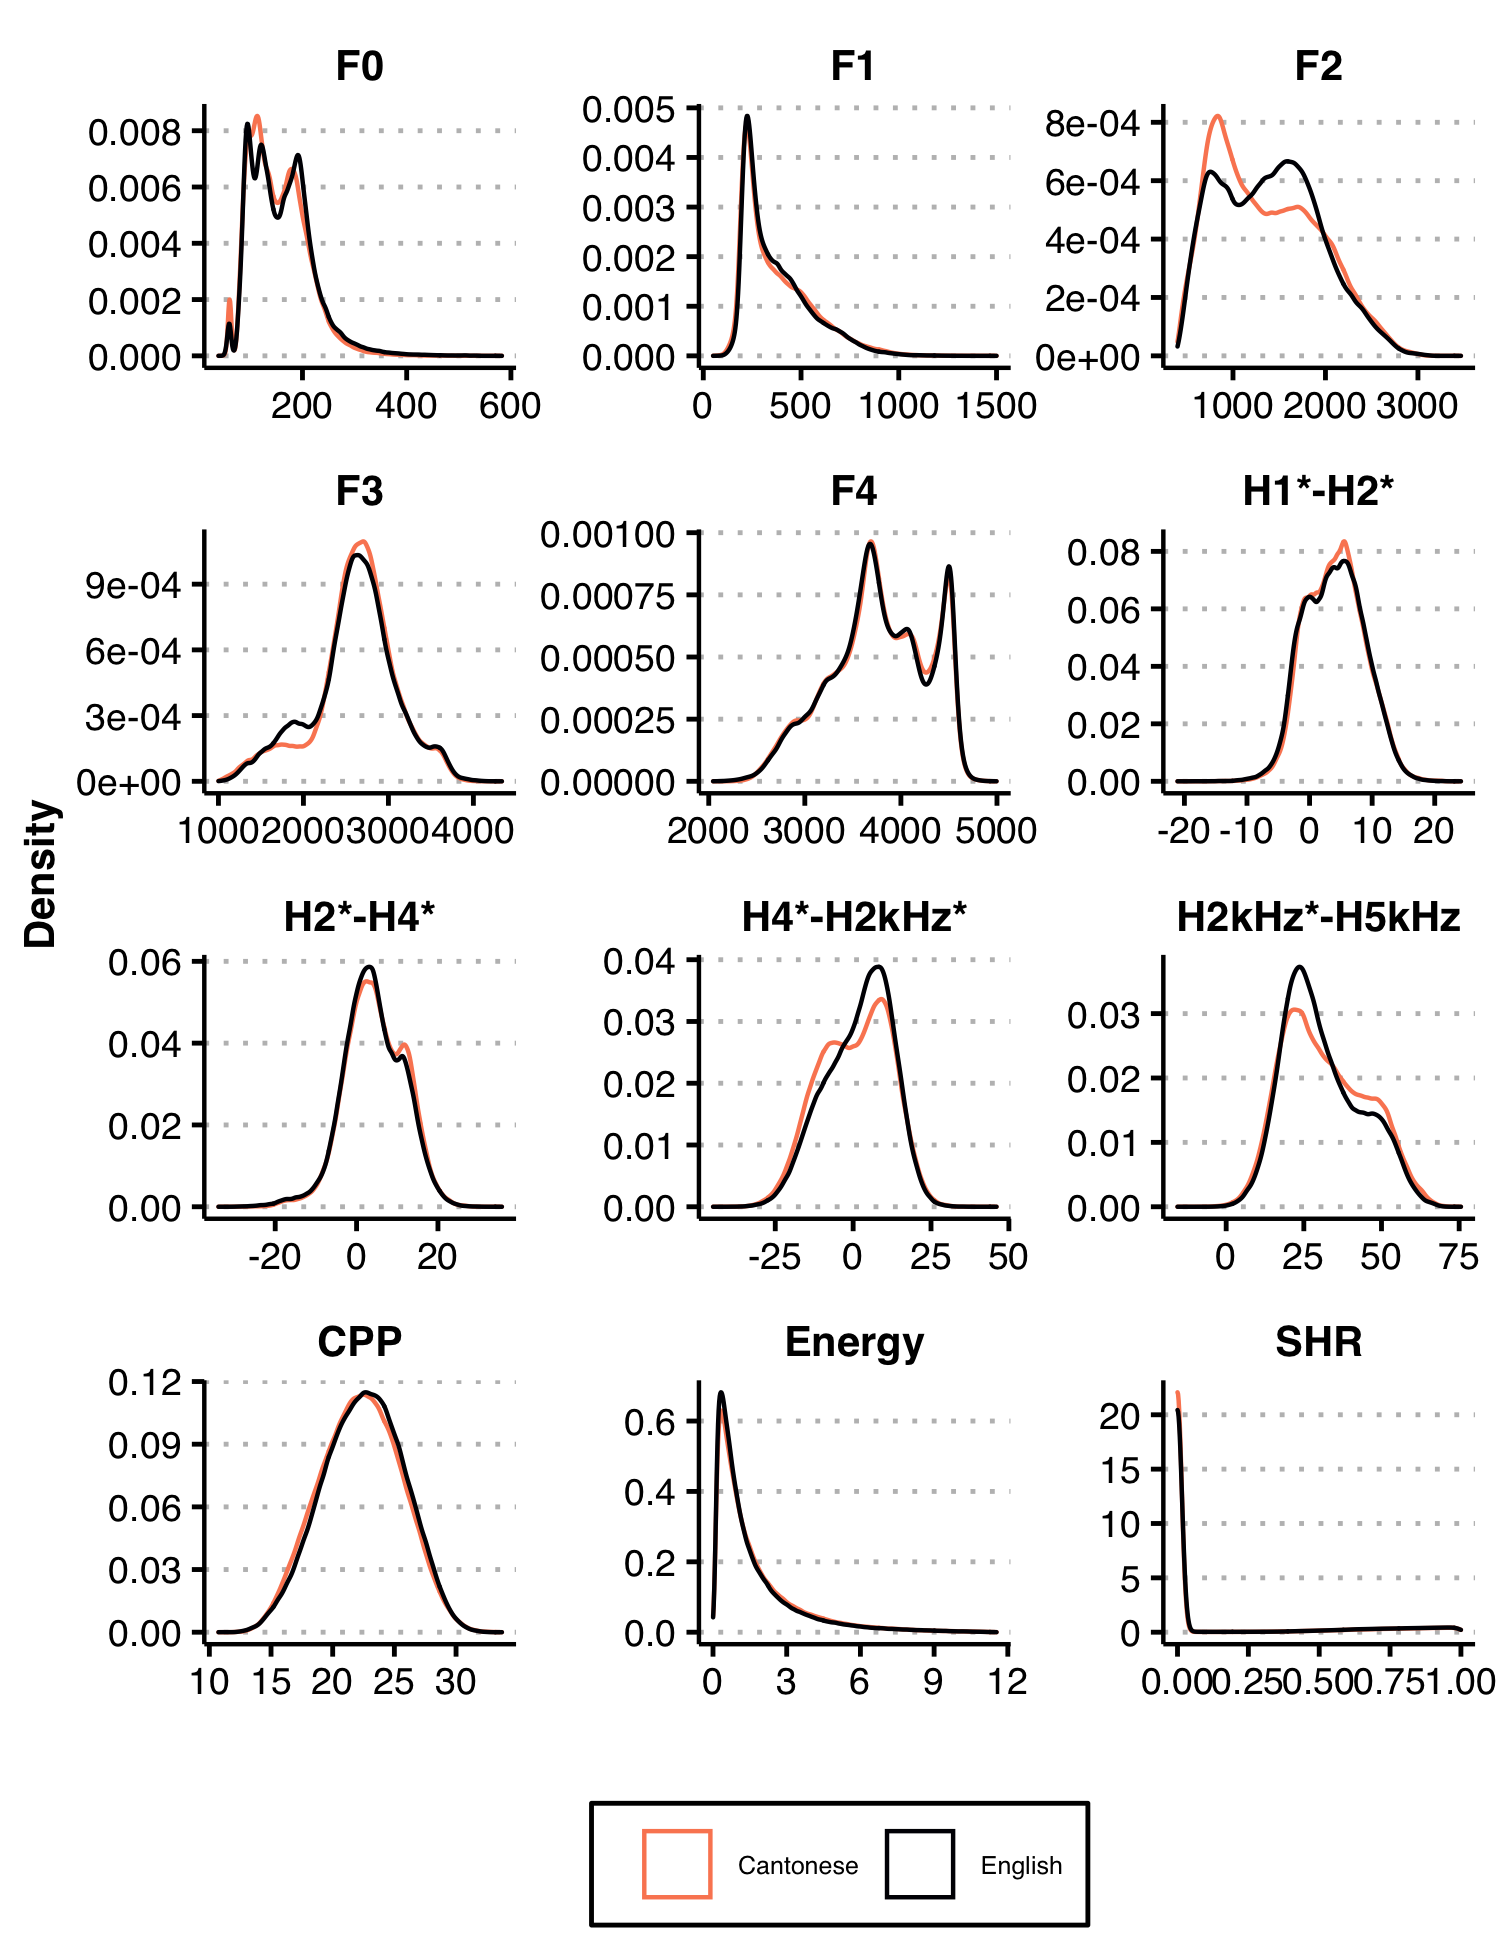
\includegraphics[width=0.9\linewidth]{figures/ch3_allmeasuresdensity_5in.png} 
    \caption{Each panel depicts a density plot that pool measurments from all talkers together to show the range of values for that measure. The x-axes each have their own scale. Language is separated out by color.}
    \label{ch3:fig:allmeasures}
    \end{center}
\end{figure}

For each acoustic measurement and talker, I conducted a Student's \textit{t}-test and calculated Cohen's \textit{d} using the \textit{lsr} package \citep{navarro_2015_lsr} in R \citep{r_2021}; this provides a high-level assessment of whether variable means differed across the two languages. These comparisons have no bearing on how a given variable \textit{varies}. Table~\ref{ch3:tab:cohend} reports counts of talkers by effect size. Notably, across all talkers and variables, only 21.1\% yielded non-trivial Cohen's \textit{d} values, though most talkers (32/34) had at least one non-trivial comparison. The distribution of these counts is depicted in Figure~\ref{ch3:fig:ntcounts}. 

\begin{table}[htbp]
\caption{This table reports counts of Cohen's \textit{d} for crosslinguistic comparisons of each of the acoustic measurements by talker. Degrees of freedom ranged between 49,274--136,644 across t-tests. For most talkers and variables, the difference in means was trivial, which is reflected in that column's high counts.}
\label{ch3:tab:cohend}
\centering
\begin{tabular}{lccc}
\toprule
         & \multicolumn{3}{c}{\textbf{Cohen's \textit{d}}} \\
         & \textbf{Trivial} & \textbf{Small} & \textbf{Medium} \\
\textbf{Variable} & \textbf{\textit{0.0--0.2}} & \textbf{\textit{0.2--0.5}} & \textbf{\textit{0.5--0.8}} \\ 
\midrule
F0	        &	21	&	10	&	3	\\
F0 s.d.	    &	34	&	-	&	-	\\
F1	        &	24	&	9	&	1	\\
F1 s.d.	    &	29	&	5	&	-	\\
F2	        &	26	&	8	&	-	\\
F2 s.d.	    &	32	&	2	&	-	\\
F3	        &	24	&	9	&	1	\\
F3 s.d.	    &	29	&	5	&	-	\\
F4	        &	30	&	3	&	1	\\
F4 s.d.	    &	28	&	6	&	-	\\
H1*--H2*	    &	18	&	15	&	1	\\
H1*--H2* s.d.	&	32	&	2	&	-	\\
H2*--H4*	    &	25	&	9	&	-	\\
H2*--H4* s.d.	&	31	&	3	&	-	\\
H4*--H2kHz* 	    &	25	&	8	&	1	\\
H4*--H2kHz*  s.d.	&	34	&	-	&	-	\\
H2kHz*--5kHz*	    &	23	&	10	&	1	\\
H2kHz*--5kHz* s.d.	&	31	&	3	&	-	\\
CPP	        &	21	&	10	&	3	\\
CPP s.d.	&	32	&	2	&	-	\\
Energy	    &	17	&	14	&	3	\\
Energy s.d.	&	18	&	16	&	-	\\
SHR	        &	31	&	3	&	-	\\
SHR s.d.	&	29	&	5	&	- \\
\bottomrule
\end{tabular}
\end{table}

\begin{figure}[htbp]
\begin{center}
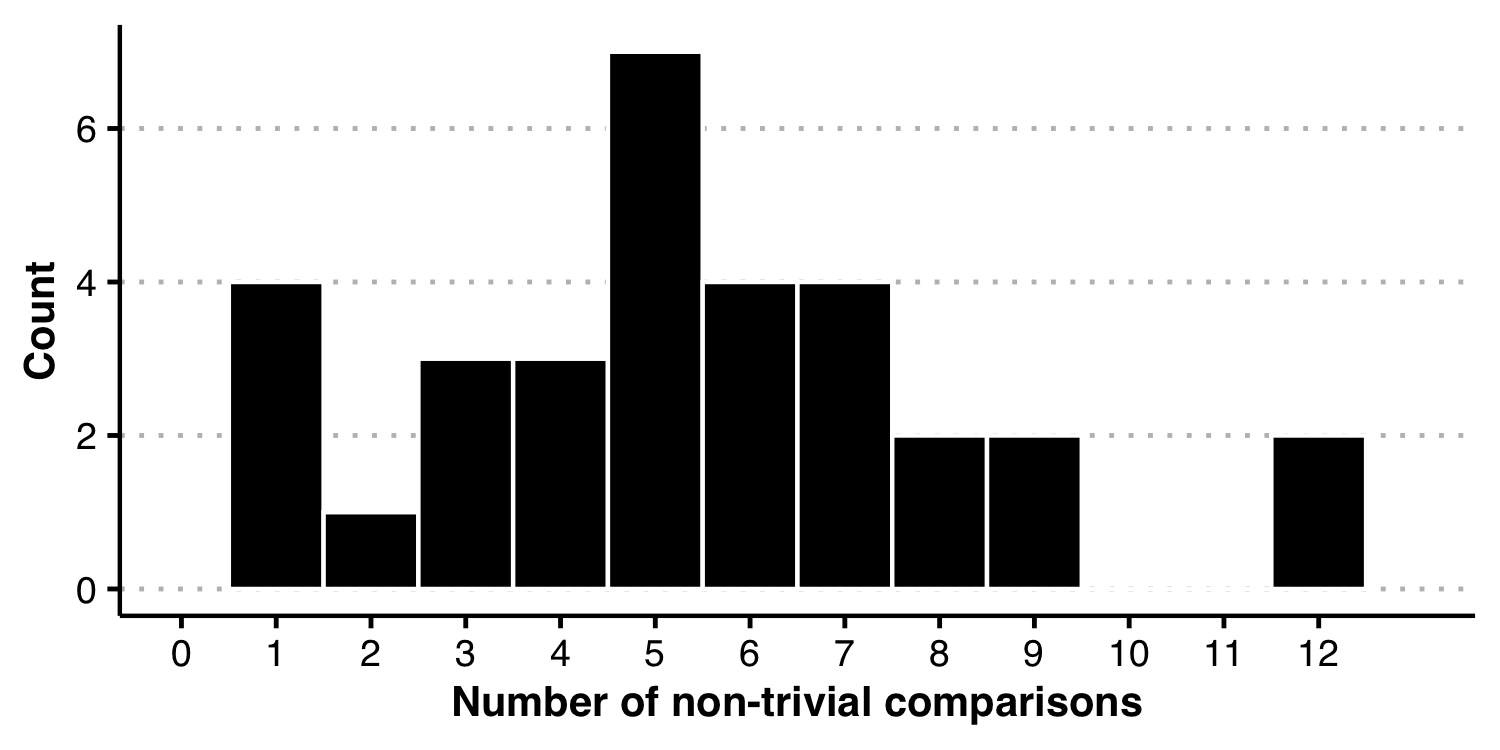
\includegraphics[width=0.875\linewidth]{figures/ch3_nontrivial_counts_by_talker_5in.png} 
\caption{A histogram summary of the number of non-trivial comparisons from Table~\ref{ch3:tab:cohend} across the 34 talkers.}
\label{ch3:fig:ntcounts}
\end{center}
\end{figure}

For the non-trivial comparisons, there were consistent patterns across languages for a handful of the variables, including F0, H4*--H2kHz, and to a lesser extent, H1*--H2**. If there was a non-trivial difference in F0 across languages, then Cantonese had a lower mean F0 than English (13/34; Female = 7), though most talkers did not exhibit a difference (21/34). This is consistent with prior findings that when a difference between English and Cantonese was found, Cantonese had a lower mean F0 for females \citep{ng_2012_ltas,altenberg_2006_f0}. I also observe this difference for a small number of males.

As for the two spectral shape measures, H4*--H2kHz was consistently lower in Cantonese when the comparison was not trivial (n=9), though most talkers did not exhibit a difference on this measure. H1*--H2* was significantly higher in Cantonese for a relatively large subset of the talkers (13/34), lower for a small number (3/34), but trivial for most (18/34). While based on a different measure than \citep{ng_2012_ltas}, this is consistent with the finding that Cantonese tends to be breathier, or English creakier---the current analysis does not distinguish between these interpretations.

For the remaining variables, while some talkers exhibited a difference in mean values, the direction of the difference varied, or relatively few talkers exhibited the difference. For example, a variable like F4 would be unlikely to vary across languages, given its association with vocal tract size. This is reflected in the relatively low count of talkers with a non-trivial difference across languages for F4. 

Other measures, such as Energy, have a high number of nontrivial comparisons but show a relatively even split for direction (Positive = 7, Negative = 10). The large spread for Energy may reflect things like speaking confidence in the two languages, which likely varies by individual \citep{jarvinen_2013_speaking}.

CPP also exhibits a split between positive (n=6) and negative (7). Higher CPP values are associated with both breathy or creaky non-modal phonation types. In this sense, a positive difference would indicate that Cantonese was more non-modal, while a negative difference would indicate that English was more non-modal. Interpreting CPP is not so straightforward, however, as it is not immediately clear which type of non-modal phonation the measure entails. Given the results of H1*--H2**, it seems clear that knowing where on the creaky-modal-breathy spectrum a given speaker falls is pertinent to interpreting this measure. CPP would likely corroborate that outcome. \hl{How much more interpretation should I add in here?}

Overall, while talkers show some clear across-language differences, these are far outnumbered by instances with no difference. The variability observed here fits in with the variable outcomes of previous work but does not necessarily fall neatly along the lines prior work would suggest that male and female talkers fall along. 

\begin{figure}[htbp]
    \begin{center}
    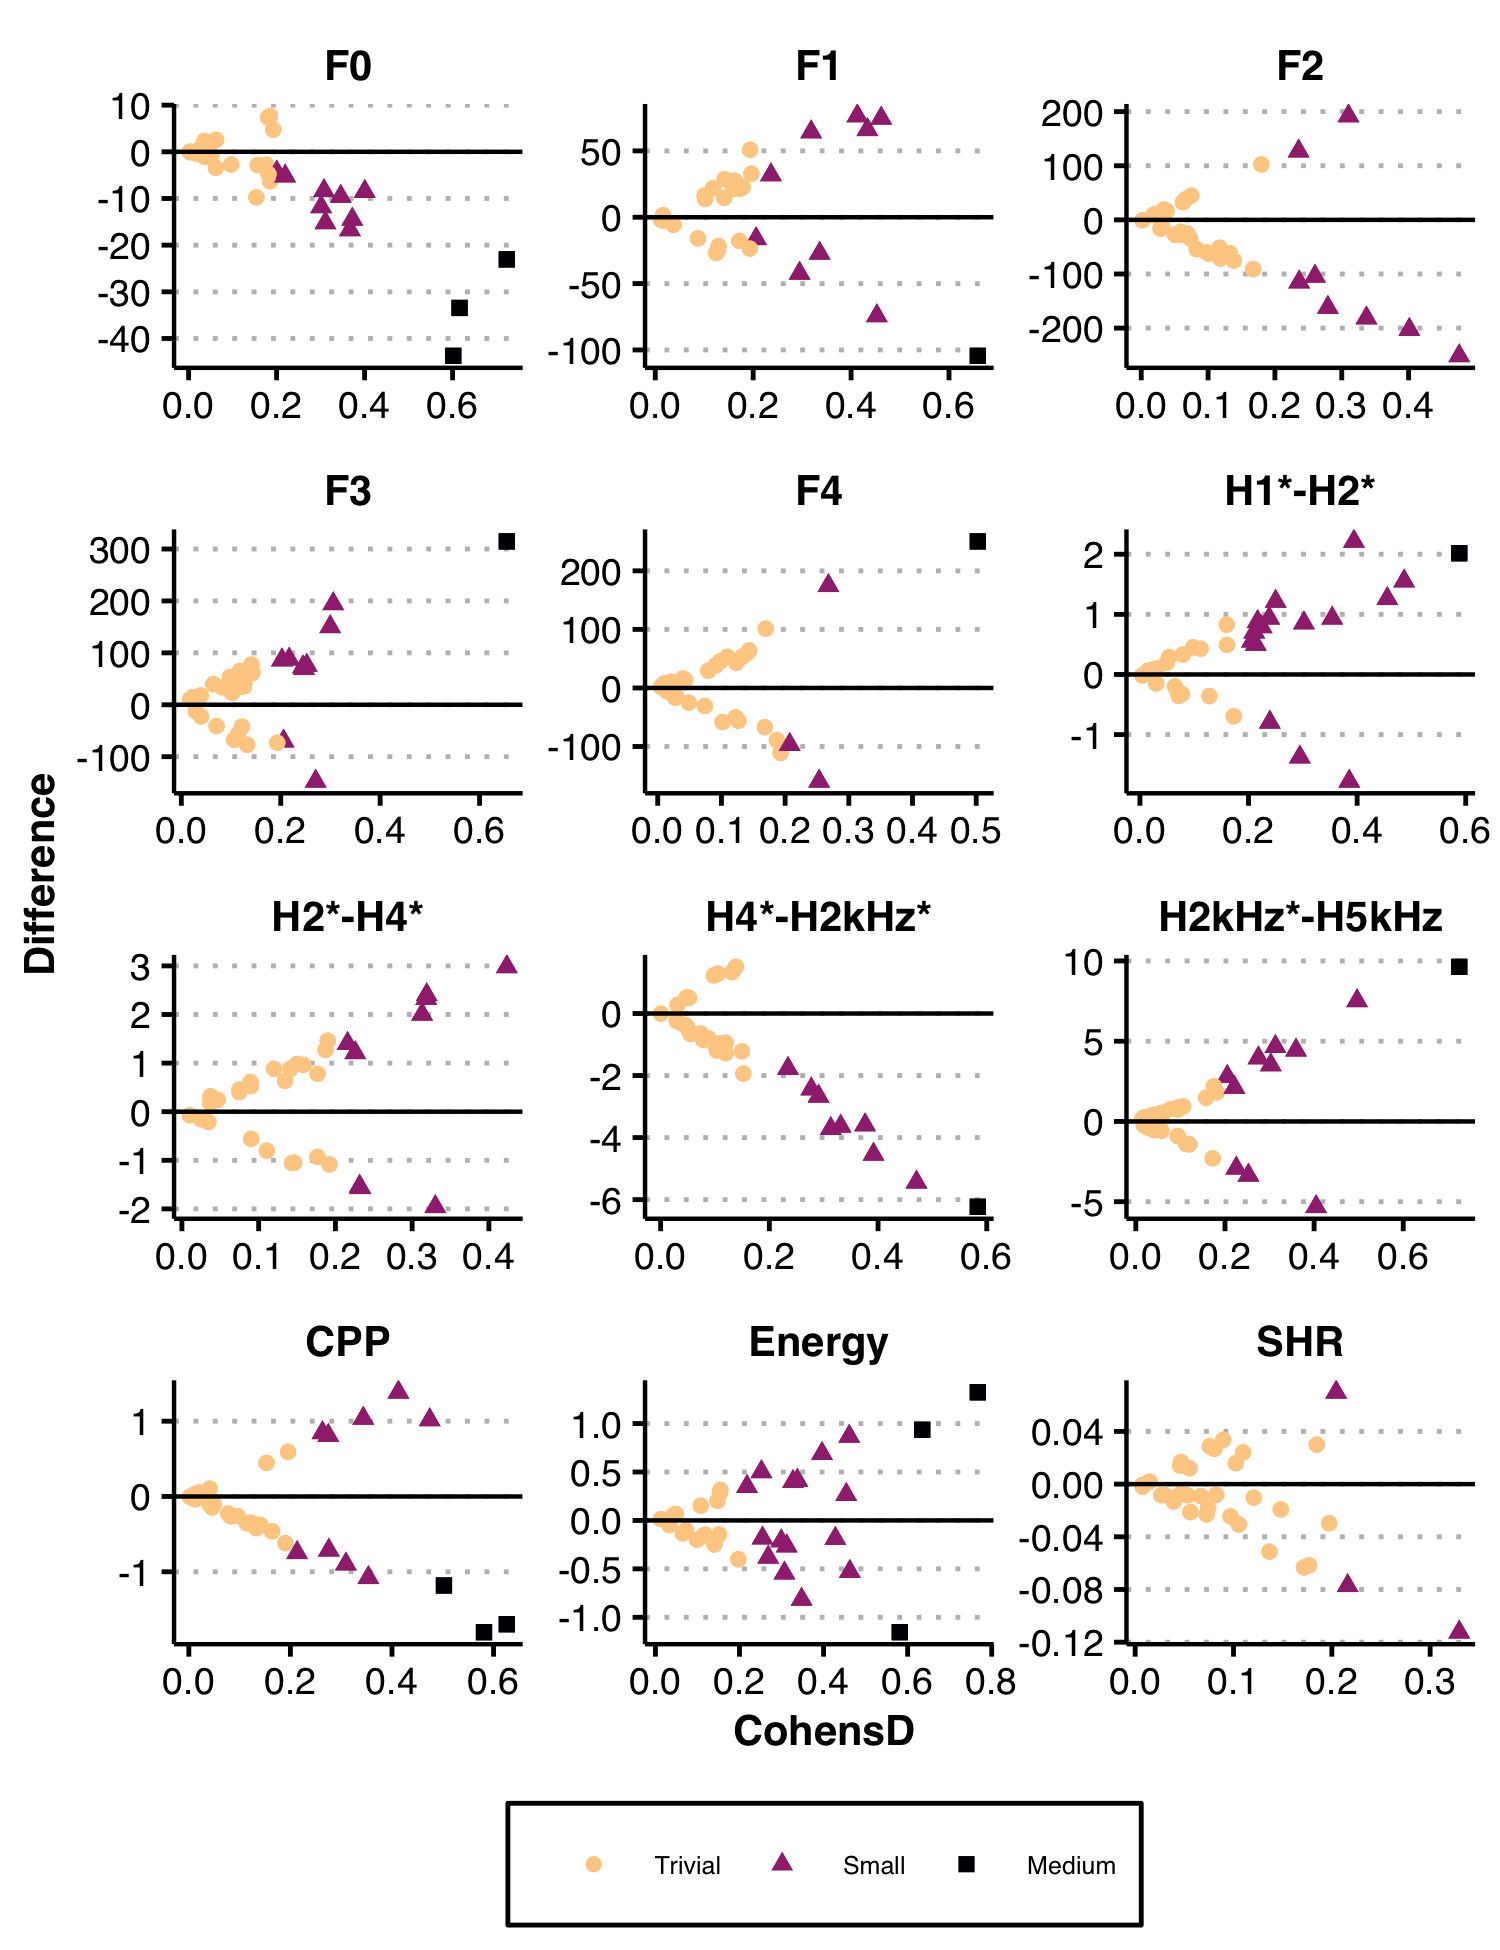
\includegraphics[width=0.9\linewidth]{figures/ch3_cohend_part1_5in.png} 
    \caption{Each panel plots Cohen's \textit{d} on the x-axis, and the difference between means from the t-tests on the y-axis. Positive values indicate a higher mean in Cantonese than English. The color reflect the levels of interpreations for Cohen's \textit{d}.}
    \label{ch3:fig:cohendmeasure}
    \end{center}
\end{figure}

\begin{figure}[htbp]
    \begin{center}
    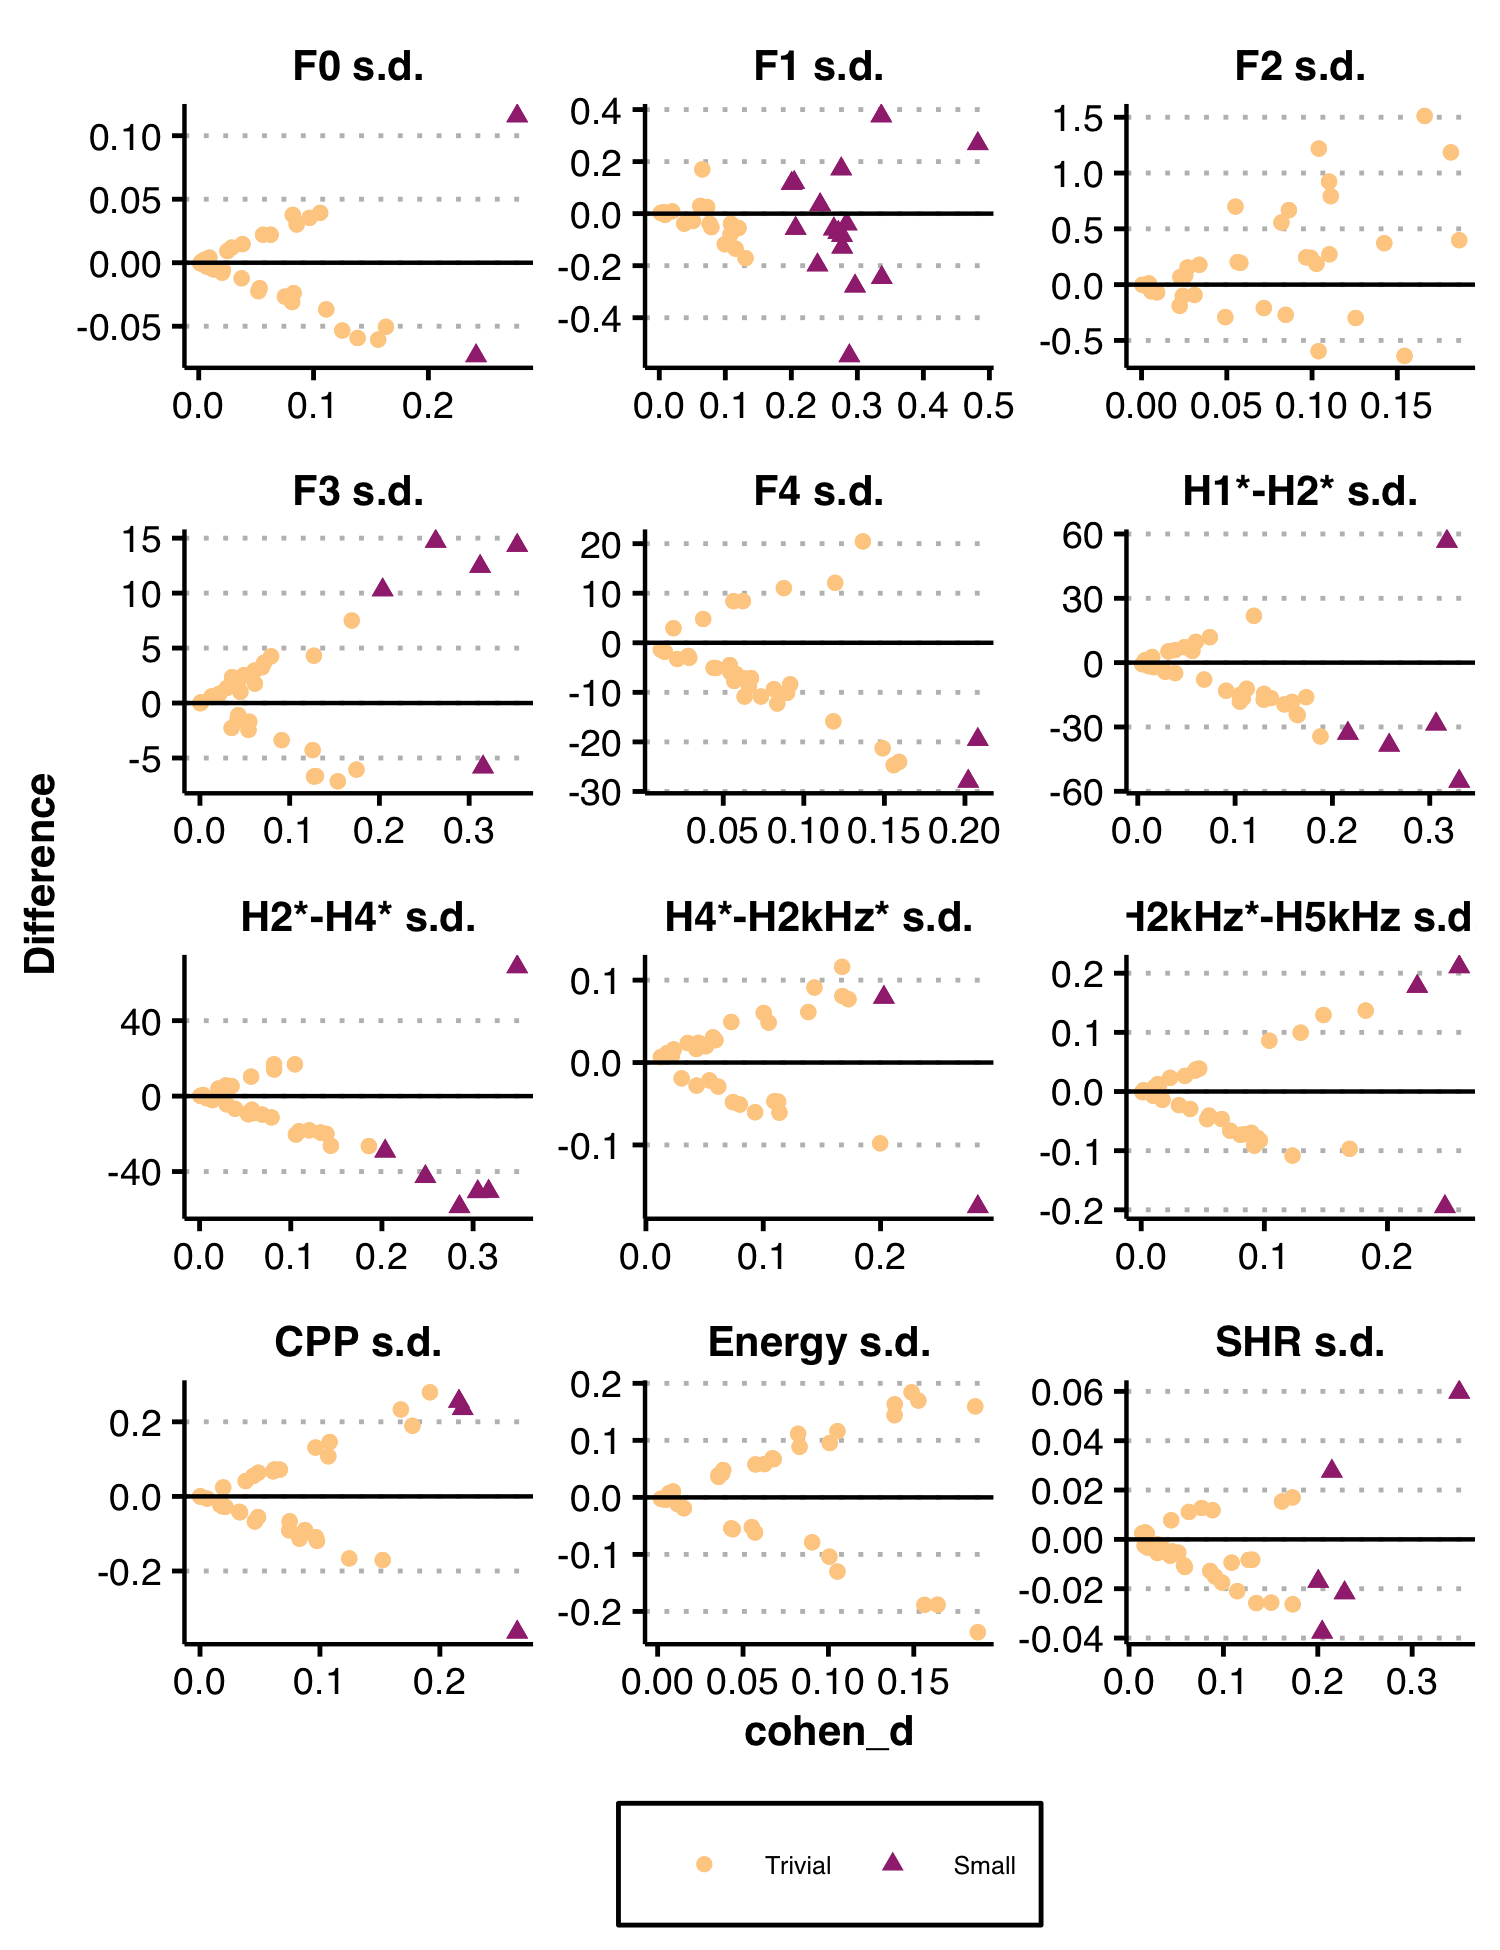
\includegraphics[width=0.9\linewidth]{figures/ch3_cohend_part2_5in.png} 
    \caption{This figure is a continuation of \ref{ch3:fig:cohendmeasure}.}
    \label{ch3:fig:cohendsd}
    \end{center}
\end{figure}

\subsection{Principal components analysis}\label{ch3:sec:pca}

\subsubsection{Methods}

Principal components analysis (PCA) is a dimensionality reduction technique appropriate for data with many potentially correlated variables. In the case of voices, distilling numerous acoustic dimensions into a smaller number of components facilitates identifying and describing the structure of voice variability. PCA provides insight into how variables pattern together in a data set. This feature of PCA is especially relevant here, as voice perception research has made it clear that individual acoustic measurements may be necessary to capture and encode a voice but may not be perceptually meaningful to listeners. What matters is how the different pieces conspire together to form a percept. 

Often, the goal of PCA is to take a large number of dimensions and extract a much smaller set to use for some additional purpose (e.g., linear regression). The focus in this chapter is on the internal structure of the components. That is, I examine what makes up components for different talkers and whether an individual's voice structure varies (or not) across languages.  

I adapt methods from work on voices \citep{lee_2019_acoustic, lee_2020_language} and faces \citep{burton_2016_faces, turk_1991_eigenfaces}. The goal of this analysis is to capture similarities or differences in the structure of each talker's voice across languages. As such, I conducted PCAs separately for each talker-language pair and compared the results of each talker's English and Cantonese PCAs. All 24 measures were standardized on a by-PCA basis before the analysis. PCAs were implemented with the \textit{parameters} package \citep{makowski_2019_parameters} in R \citep{r_2021}, using an oblique \textit{promax} rotation to simplify the factor structure, as the measurements reported in the previous section were expected to be somewhat correlated given prior findings \citep{lee_2019_acoustic} and a broader understanding of how different acoustic measures align with one another \citep{kreiman_2014_theory, kreiman_2021_validating}.

Each PCA included the number of components for which all resulting eigenvalues were greater than 0.7 times the mean eigenvalue, following \citeauthor{jolliffe_2002_pca}'s \citeyearpar{jolliffe_2002_pca} recommended adjustment to the Kaiser-Guttman rule. This rule was used in place of a more sophisticated test (e.g., broken sticks), as it is not detrimental to this exploratory analysis to err on the side of including marginal components. Additionally, across each of the components, only loadings with an absolute value of 0.45 or higher were interpreted \citep{lee_2019_acoustic, tabachnick_2013_statistics}. While \citet{lee_2019_acoustic} use a threshold of 0.32, \citet{tabachnick_2013_statistics} note that higher loadings indicate that a particular variable is a better measure of the component, with 0.32 corresponding to poor (but still interpretable) overlap between the variable and the component. The guidelines in \citet{tabachnick_2013_statistics} indicate that loadings of 0.45 correspond to fair, 0.55 to good, 0.63 to very good, and 0.71 and above to excellent. Given the large number of components and loadings in this analysis, only loadings over the fair threshold are interpreted.

\subsubsection{Results}\label{ch3:sec:pca_results} 

The PCAs across both languages for all 34 talkers resulted in 10--14 components and accounted for 74.9--82.7\% of the total variation. Half of the talkers had the same number of components for each language (17 of 34). Of the remainder, 16 of the 34 talkers had a difference of one in the number components, and only one had a difference of two. Talkers had 4--11 identical component configurations across their languages (M$=$7.82). These shared components represent 33.3\%--91.7\% of the total components for talkers (M$=$66.7\%). The numbers comprising these summary statistics are provided in Table \ref{ch3:tab:componentcount}. While this already indicates a substantial amount of shared lower-dimensional structure across languages, it likely underestimates the actual shared structure. The reason is that similarity of component structure is not taken into account (i.e., a component of F2, F3, and F4 versus a component with just F2 and F3), as is the case in Section \ref{ch3:sec:cca}. 

\begin{table}[htbp]
    \caption{The number of components and the variance accounted for is listed for each PCA. The last column indicates the number of identical components across langauges.}
\label{ch3:tab:componentcount}
\centering
{\footnotesize 
    \begin{tabular}{llllll}
    
    \toprule
     & \multicolumn{2}{l}{\textbf{Cantonese}} & \multicolumn{2}{l}{\textbf{English}} &  \\
    \textbf{Talker} & \textbf{N} & \textbf{Variance} & \textbf{N} & \textbf{Variance} & \textbf{Identical N} \\
    \midrule
    \textbf{VF19A} & 11 & 0.77 & 12 & 0.80 & 8 \\
    \textbf{VF19B} & 12 & 0.78 & 12 & 0.78 & 8 \\
    \textbf{VF19C} & 12 & 0.78 & 12 & 0.79 & 9 \\
    \textbf{VF19D} & 13 & 0.81 & 13 & 0.78 & 9 \\
    \textbf{VF20A} & 11 & 0.78 & 12 & 0.79 & 6 \\
    \textbf{VF20B} & 13 & 0.81 & 12 & 0.82 & 8 \\
    \textbf{VF21A} & 12 & 0.78 & 12 & 0.80 & 6 \\
    \textbf{VF21B} & 12 & 0.78 & 12 & 0.80 & 8 \\
    \textbf{VF21C} & 14 & 0.83 & 13 & 0.83 & 10 \\
    \textbf{VF21D} & 12 & 0.79 & 12 & 0.81 & 9 \\
    \textbf{VF22A} & 11 & 0.78 & 12 & 0.80 & 7 \\
    \textbf{VF23B} & 12 & 0.78 & 12 & 0.78 & 8 \\
    \textbf{VF23C} & 12 & 0.79 & 12 & 0.80 & 7 \\
    \textbf{VF26A} & 12 & 0.78 & 13 & 0.80 & 7 \\
    \textbf{VF27A} & 11 & 0.79 & 11 & 0.77 & 8 \\
    \textbf{VF32A} & 12 & 0.78 & 11 & 0.76 & 8 \\
    \textbf{VF33B} & 12 & 0.77 & 12 & 0.79 & 9 \\
    \textbf{VM19A} & 12 & 0.78 & 11 & 0.76 & 5 \\
    \textbf{VM19B} & 11 & 0.80 & 12 & 0.80 & 6 \\
    \textbf{VM19C} & 11 & 0.76 & 11 & 0.78 & 6 \\
    \textbf{VM19D} & 13 & 0.80 & 14 & 0.82 & 10 \\
    \textbf{VM20B} & 12 & 0.80 & 11 & 0.76 & 9 \\
    \textbf{VM21A} & 10 & 0.78 & 11 & 0.79 & 5 \\
    \textbf{VM21B} & 11 & 0.79 & 11 & 0.76 & 9 \\
    \textbf{VM21C} & 12 & 0.80 & 12 & 0.77 & 9 \\
    \textbf{VM21D} & 11 & 0.75 & 12 & 0.77 & 7 \\
    \textbf{VM21E} & 10 & 0.74 & 12 & 0.80 & 7 \\
    \textbf{VM22A} & 12 & 0.77 & 13 & 0.83 & 11 \\
    \textbf{VM22B} & 12 & 0.79 & 12 & 0.79 & 7 \\
    \textbf{VM23A} & 12 & 0.81 & 12 & 0.79 & 4 \\
    \textbf{VM24A} & 11 & 0.77 & 11 & 0.76 & 8 \\
    \textbf{VM25A} & 12 & 0.81 & 12 & 0.77 & 11 \\
    \textbf{VM25B} & 11 & 0.74 & 12 & 0.76 & 7 \\
    \textbf{VM34A} & 11 & 0.77 & 12 & 0.81 & 10 \\
    \bottomrule
    \end{tabular}
}
\end{table}

To assess whether talkers exhibit the same structure in voice variability across their languages, I first consider the patterns present across the different PCAs. This provides context for understating what unique structural characteristics in talkers' voices looks like. To this end, I briefly summarize common patterns across PCA components, regardless of how much variance they account for, as the difference is often quite small. Figure~\ref{ch3:fig:VF32A} shows all of the components of participant VF32A's Cantonese and English PCAs, illustrating some examples of how components can vary (or not) across languages. It also highlights the importance of not attributing too much value to the ordering of components, but rather to their composition and variance accounted for.

\begin{figure}[htbp]
\begin{center}
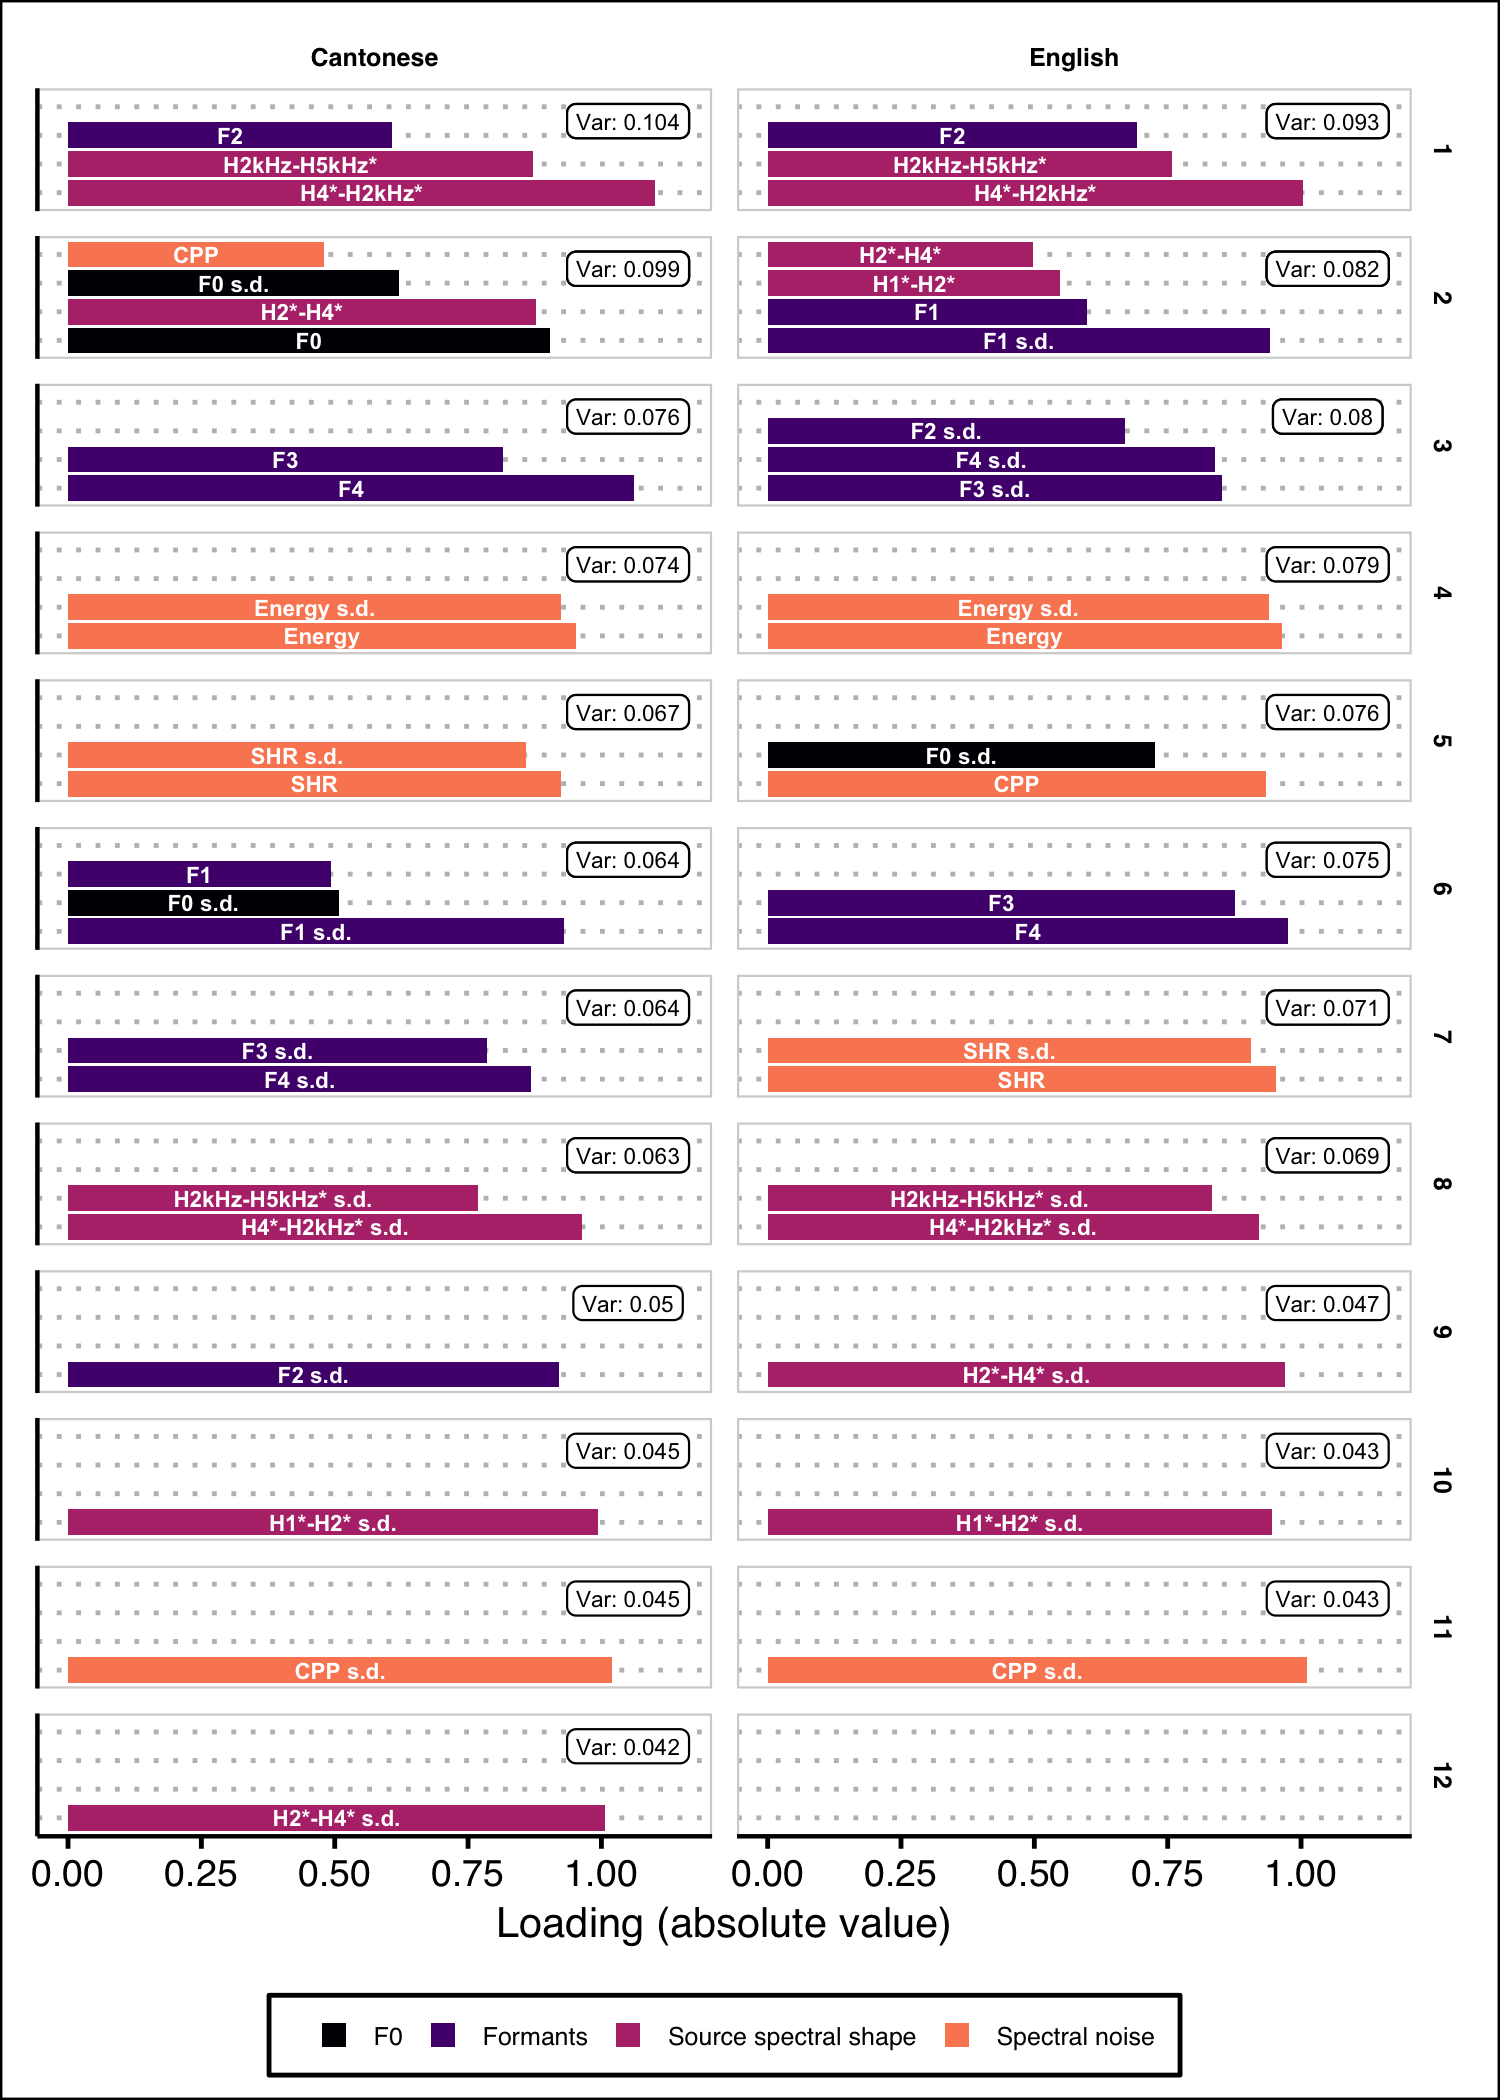
\includegraphics[width=0.8\linewidth]{figures/ch3_pca_vf32a_vert5in.png} 
\caption{In this depiction of the components of VF32A's Cantonese and English PCAs, loadings are represented by bar height and are labelled with the variable name; color represents conceptual groupings; and, the component's variance is superimposed.}
\label{ch3:fig:VF32A}
\end{center}
\end{figure}

Broadly, there were many similarities in component composition across talkers and languages. The following paragraphs summarize the components that were present in every PCA, regardless of talker or language. The shared component accounting for the most variation across talkers had a core structure consisting of F2 and H4*-H2kHz*. These usually went along with H2kHz*-H5kHz* (Cantonese = 34, English = 31), and occasionally with F3 and F4 (Cantonese = 3, English = 3). In a similar vein, all talkers had a component consisting of H4*-H2kHz* s.d. and H2kHz*--H5kHz* s.d., though it accounted for a smaller proportion of the total variation. \hl{Should I describe what these mean here? Or in the discussion?}

In the case of the moving standard deviation parameters, there were a few common configurations. Formant s.d. parameters often co-occurred. In both languages, the component typically consisted of F3 s.d. and F4 s.d. (Cantonese = 32, English = 26), though a subset of these cases also included F2 s.d. (Cantonese = 6, English = 10). In the case of spectral shape, the variable for H2*--H4* s.d. commonly occurred alone (Cantonese = 18, English = 18) or in combination with H1*--H2* s.d. (Cantonese = 13, English = 14). While the formant and spectral shape moving standard deviations often exhibited these common patterns, variables in these categories were just as likely to pattern in more idiosyncratic ways, loading alongside each other, F0, formants, and spectral measures. This kind of variability is not readily summarizable. 

The spectral noise parameters had a relatively consistent component structure across talkers and languages. Energy and Energy s.d. consistently loaded on the same component and were sometimes accompanied by F0 (Cantonese = 6, English = 2) and F0 s.d. (Cantonese = 1). CPP s.d. occurred consistently on its own component for all English PCAs, and 31 of the Cantonese PCAs. In the remaining three Cantonese PCAs, CPP s.d. was accompanied by CPP (n=1) or H1*-H2* s.d. (n=2). CPP patterned less consistently but was most often accompanied by F0 s.d. (Cantonese = 19, English = 14). SHR and SHR s.d. exclusively loaded together for 31 talkers in each language and SHR by itself for a single talker per language. The pair was sometimes accompanied by H1*-H2* (Cantonese = 2, English = 2), H2*-H4* (English = 1), or F0 (English = 3). 

While this covers many of the variables that went into the PCAs, F0 is notably sparse in the above paragraphs. While F0 s.d. was fairly consistent in emerging either with CPP (Cantonese = 21, English = 17) or alone (Cantonese = 9, English = 10), the same cannot be said for F0. No particular component structure with F0 occurred more than six times, and across the wide range of configurations, F0 was accompanied by all kinds of variables: F0 s.d., H1*--H2*, H1*--H2* s.d., H2*--H4*, F1 s.d., F4 s.d., CPP, Energy, Energy s.d., and SHR, SHR s.d. The lack of consistency in F0 across talkers is notable for a few reasons. First, F0 plays a major role in prior work on voice production and perception, given its salience as an acoustic dimension \citep{perrachione_2019_judgments}. A second reason for it being notable comes from Lee and colleagues' work, where F0 emerged as an important feature of acoustic voice variation structure in English spontaneous speech \citep{lee_2019_spontaneous} and Korean sentence reading \citep{lee_2020_language}, but not for English sentence reading \citep{lee_2019_acoustic}. 

On the whole, variables emerged on a single component. That is, very few variables had complex loading structures. Across talkers, only three had complex loading structures for H2*--H4* in each language. F0 and F0 s.d. participated in complex loadings for a single English talker, and twice in the Cantonese PCAs. The remaining variables that participated in complex loading structures only occurred in one or two PCAs across all talkers and languages. This means that for a given PCA, the interpretation of components is reasonably straightforward, even if drawing generalizations over the full group is not. 

There were additional components (not reported here) that were shared by less than half of the talkers. A full list of component configurations, along with the number of occurrences and range of variation accounted for is provided in the supplementary materials. \hl{Well... it will be! Also, would a table in this section help with interpretation? Or is prose plus supplementary materials good enough?}

In summary, this PCA analysis found a greater amount of component structure overlap than was reported in \citet{lee_2019_acoustic}. At the same time, idiosyncratic variation was still readily apparent in the PCAs, both in how variables co-occur, as well as in how much variance is accounted for by the different components. Additionally, it is important to remember that these PCAs represent the lower dimensional structure of the voices they measure. Considering that the total variance unaccounted for by the PCAs ranges from 17.3\%--25.1\%, this unaccounted for variability may also be idiosyncratic in nature. 

\subsection{Canonical redundancy analysis}\label{ch3:sec:cca}

\subsubsection{Methods}

To assess whether variation in a talker's voice is structurally similar across both languages, I compare PCA output from both languages by calculating redundancy indices in a canonical correlation analysis \citep[CCA][]{stewart_1968_canonical, jolliffe_2002_pca}. CCA is a statistical method used to explore how groups of variables relate to one another. The two sets of variables are transformed such that the correlation between the rotated versions is maximized. This is useful here, as a talker may have similar components in their English PCA and Cantonese PCA, but these components might not necessarily be in the same order, even if they account for comparable amounts of variance.

Redundancy is a relatively simple way to characterize the relationship between the loadings matrices of two PCAs---the two sets of variables under consideration here. For example, the two redundancy indices represent the amount of variation in a talker's Cantonese PCA output that can be accounted for via canonical variates by their English PCA output and vice versa. Notably, the two redundancy indices are not symmetrical \citep{stewart_1968_canonical}. This is particularly relevant in cases where the PCAs comprise different numbers of components, as determined by the stopping rule described above. The PCA with more components will likely account for more of the variation in a PCA with fewer components than the reverse.

Redundancy indices were computed for all pairwise combinations, including cases where similar values were expected (same talker, different language) and cases where dissimilarity was anticipated (different talker and language). Considering that the PCA analyses capture the lower-dimensional structure within each language, these redundancy indices effectively reflect the degree to which the lower-dimensional structure of acoustic voice variability is shared across a talker's two languages.

\subsubsection{Results}

Redundancy indices for within-talker comparisons ranged from 0.80 to 0.97, (\textit{Mdn} = 0.92, \textit{M} = 0.91, \textit{SD} = 0.04) and are displayed in Figure~\ref{ch3:fig:redundancy}, with the two redundancy indices for a given pairwise comparison plotted against one another. Comparisons across talkers within-language ranged from 0.64 to 0.96 (\textit{Mdn} = 0.83, \textit{M} = 0.83, \textit{SD} = 0.5). Comparisons across both talkers and languages ranged from 0.64 to 0.97 (\textit{Mdn} = 0.83, \textit{M} = 0.83, \textit{SD} = 0.5). Within-talker values were confirmed to be higher than across-talker comparisons, per a Welch's t-test (\textit{t}(70.93) = $-$17.35, \textit{p} $<$ 0.001, d = 1.77). A second Welch's t-test testing the same versus different language for the across talker comparisons did not find a difference between those groups (\textit{t}(4485.9) = $-$1.53, \textit{p} = 0.13, d = 0.05). 

While the across-talker comparisons were generally lower than the within-talker ones, the redundancy indices are overall still relatively high. The high values are not unexpected. As PCA is a dimensionality reduction technique, the discarded components almost certainly contain idiosyncratic variation. Moreover, and following from Section~\ref{ch3:sec:pca_results}, there were a substantial number of commonly occurring patterns across talkers and languages. Together, this supports the conceptualization of a voice space comprising a shared structure---as in the case of the prototype account---where voices can only deviate from one another so much.

\begin{figure}[htbp]
\begin{center}
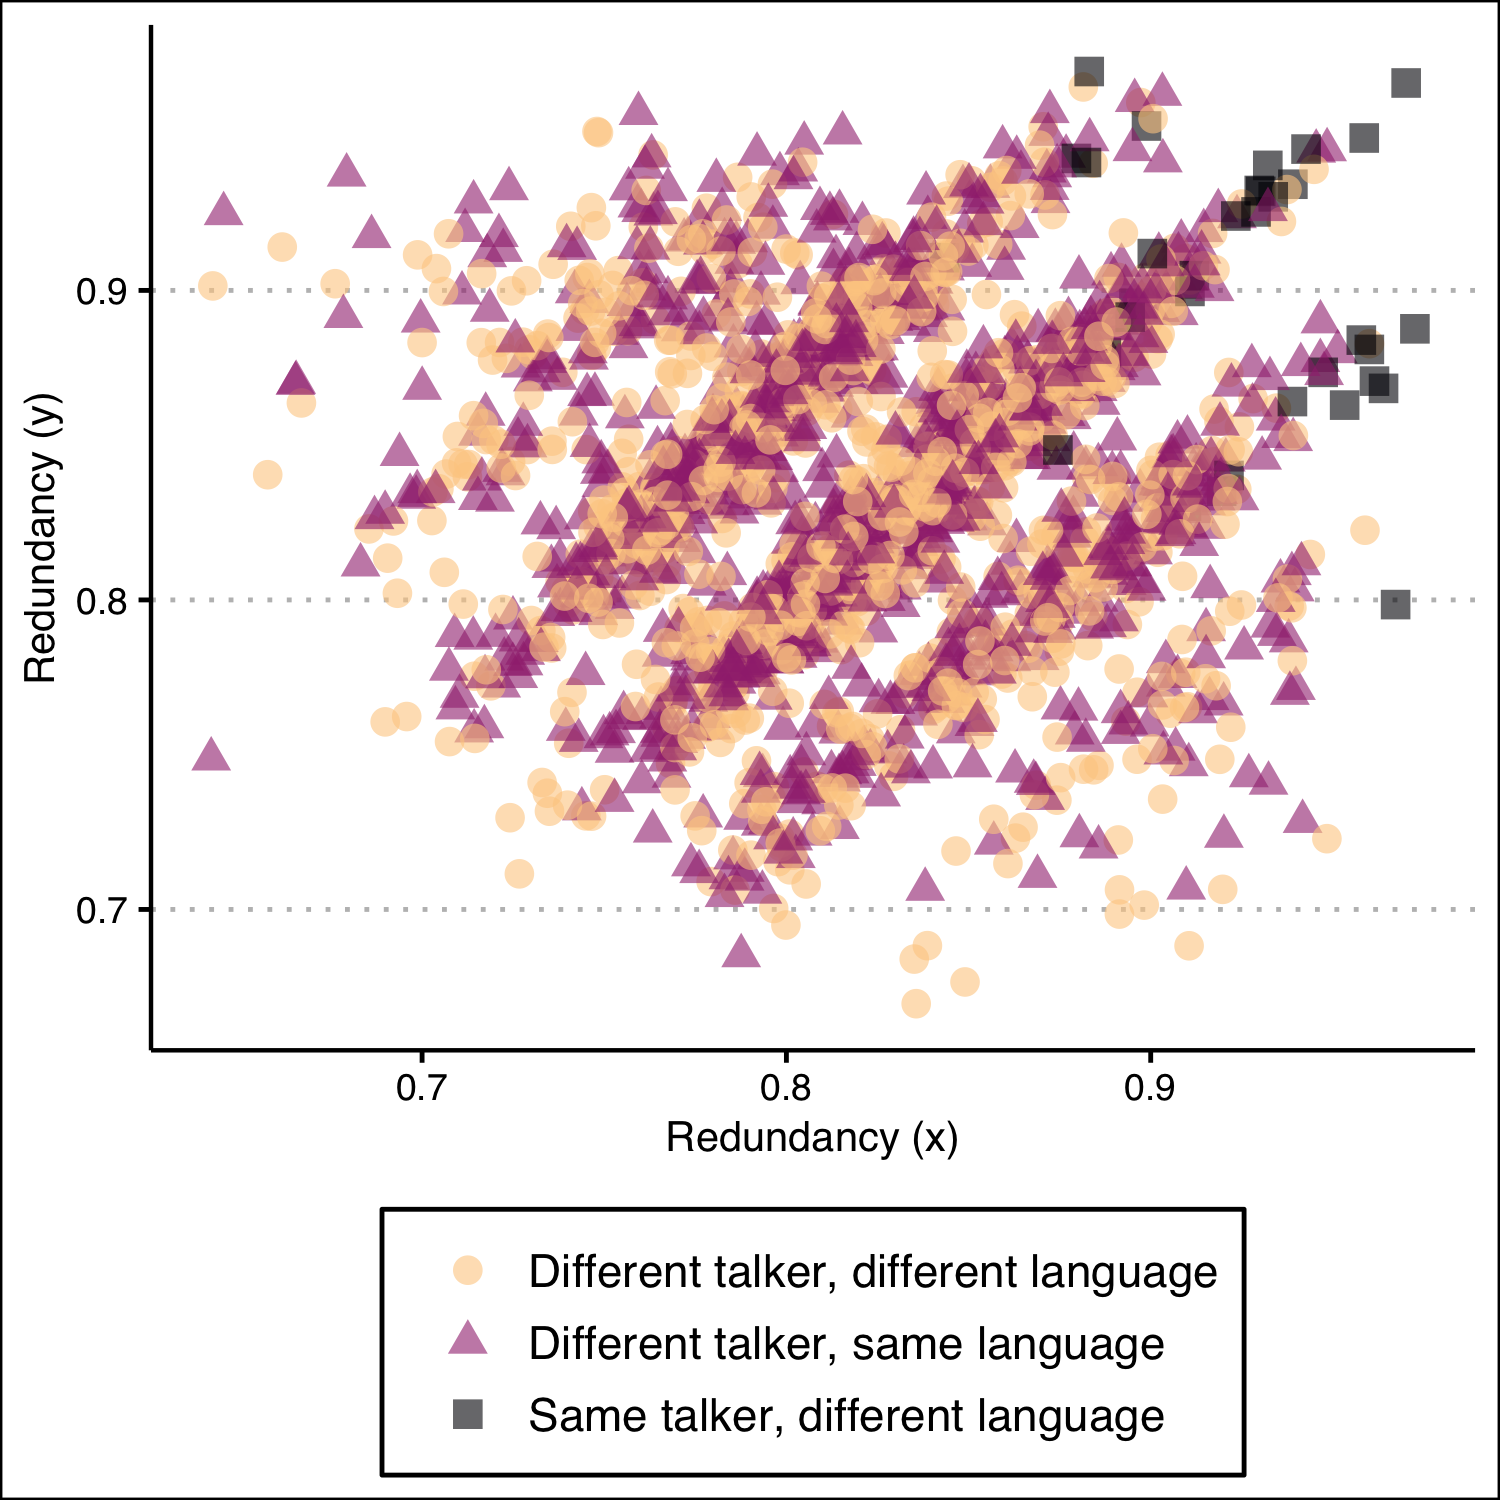
\includegraphics[width=0.9\linewidth]{figures/ch3_redundancy.png} 
\caption{The relationship between the two redundancy indices for three different types of comparisons. Within-talker comparisons are represented by the black squares and are clearly clustered at the top right.}
\label{ch3:fig:redundancy}
\end{center}
\end{figure}

\subsection{Passage length analysis}\label{ch3:sec:passagelength}

As previewed in the introduction, passage length is an important consideration in the principal components and canonical redundancy analyses. It represents one possible reason why the results presented in this chapter differ from prior work. To examine the role of passage length, I conducted multiple PCAs for each talker and language combination, such that each PCA captured a progressively longer portion of the overall interview, using passage lengths comprising sample sizes of 500, 2000, 4500, 8000, 12500, 18000, 24500, 32000, 40500, 50000, 60500, and 72000. As the total number of samples per interview ranged from 20124 to 74638, there were six to 12 total PCAs per interview, depending on its maximum possible passage length. While the step sizes were somewhat arbitrarily selected, the goal was to give a more granular perspective on the lower end, while still covering the upper tail. Redundancy was expected to level off somewhere in the middle, as talkers should eventually cover their range of variability in a given style.

In these PCAs, the number of components was fixed at 10, the lowest number found in Section \ref{ch3:sec:pca_results}. This was done to put the PCAs on more equal footing in the subsequent analysis, given the asymmetries in CCA when different numbers of components were present. For each interview, the canonical redundancy indices were calculated for each talker and language combination, comparing PCAs for each passage length to the PCA for the longest passage length. All of this was done on a within-language and within-talker basis. The final comparison thus has perfect redundancy, as the longest PCA for a given interview is compared to itself.

\begin{figure}[htbp]
    \begin{center}
    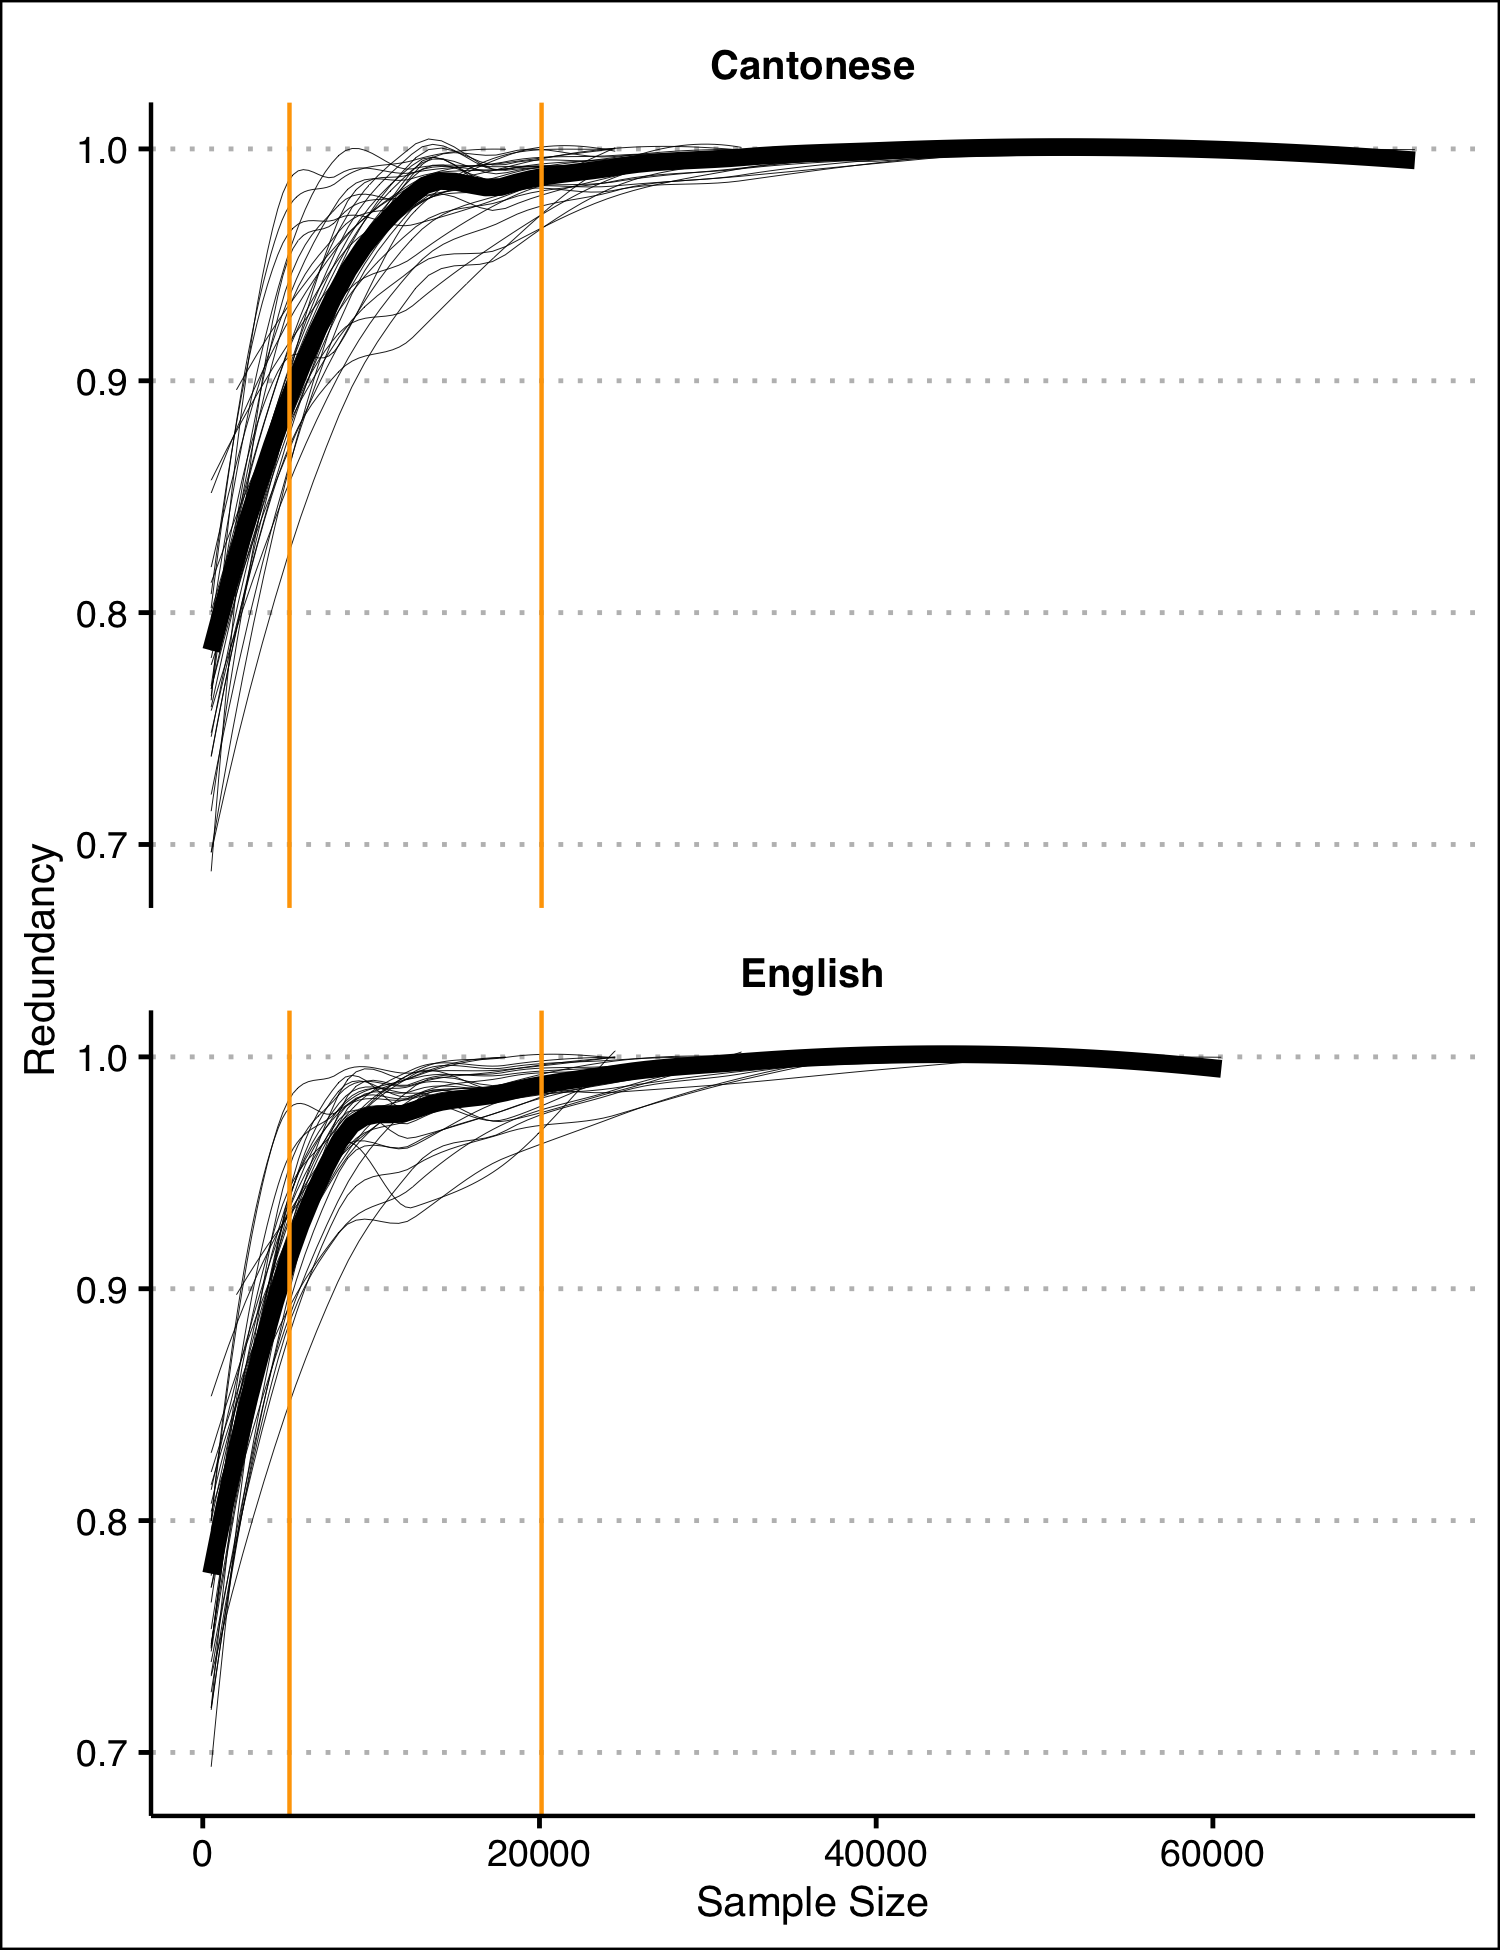
\includegraphics[width=0.85\linewidth]{figures/ch3_passagelength.png} 
    \caption{Passage length redundancy indices are plotted against the sample size of the smaller PCA. Smoothed curves show a rapid increase in redundancy followed by a levelling off between the vertical orange lines, which represent the sample sizes used in prior work (x = 5000) and the present study (x = 20124).}
    \label{ch3:fig:passagelength}
    \end{center}
\end{figure}

Figure \ref{ch3:fig:passagelength} plots polynomial smooths for each interview, with superimposed mean smooths. The x-axis represents the sample size of the shorter passage length in the comparison. The y-axis represents an average of the two redundancy indices. The vertical line at 5000 represents the average sample size from \citet{lee_2019_acoustic}. The vertical line at 20124 represents the sample size used in Sections \ref{ch3:sec:pca} and \ref{ch3:sec:pca_results}. While there are some gains in sample sizes above the second vertical line, they are comparatively small. It is readily apparent from this plot that the sample size used for PCAs in this chapter was sufficient to capture most of the range of talkers' within-interview variability. As the leveling-off point likely varies across speech styles, it is not immediately apparent whether the sample size in \citet{lee_2019_acoustic} sufficiently captured the range of talker variability and thus may not adequately capture the structure of their variability. 

\section{Discussion and conclusion}\label{ch3:sec:discussion}

This chapter examines spectral properties and structural similarities in an individual's voice across two languages. To this end, it uses conversational interviews from the SpiCE corpus of speech in Cantonese and English, described in Chapter \ref{ch:Corpus}. The analyses presented in this chapter cover three different exploratory approaches to the question of understanding crosslinguistic (dis)similarity in bilingual voices. Section \ref{ch3:sec:comparison} takes a coarse perspective, comparing overall distributions using \textit{t}-tests and Cohen's \textit{d} values. This approach follows from a body of literature focused on crosslinguistic comparisons of acoustic measurements---primarily F0---using means, ranges, and standard deviations to describe how voices differ (or not). Section \ref{ch3:sec:pca} replicates \citeauthor{lee_2019_acoustic}'s \citeyearpar{lee_2019_acoustic} methods for drilling down into the structure of acoustic voice variation using PCAs and extends it to the case of bilingual speech. Section \ref{ch3:sec:cca} builds on the PCAs and introduces canonical redundancy as a metric for objectively assessing crosslinguistic similarity from the output of two PCAs. These methods are then extended in Section \ref{ch3:sec:passagelength} to demonstrate that the analysis used a sufficiently large sample.

A clear result in this chapter is that the bilinguals studied here exhibit similar spectral properties and similar lower-dimensional structure in their acoustic voice variation. This similarity is most apparent on a within-talker basis but still present across talkers and languages, despite substantial segmental and suprasegmental differences across English and Cantonese \citep{matthews_2013_cantonese}. In this sense, the SpiCE corpus talkers appear to have the same ``voice'' in each of the two languages. This outcome supports the characterization of voices as auditory faces. The face-voice comparison is especially apt if you take into account findings that talkers' faces vary across languages, as evidenced by work demonstrating that lip movement patterns alone are sufficient for humans and machines to identify and discriminate between spoken languages \citep{afouras_2020_now, sotofaraco_2007_discriminating}. Voices and faces are highly similar across languages but are not necessarily identical---this leaves room for individuals who are familiar with both the individuals and languages in question to excel at perceptual tasks in both domains.

It is reassuring that the results from the first two approaches used here reflect prior findings. For example, when there was a difference for measures like F0 or H1*--H2*, it tended to mirror expectations from the literature that Cantonese tends to have lower pitch and breathier voice quality than English \citep{ng_2012_ltas, ng_2010_voice}. At the same time, most talkers did not exhibit a meaningful difference, validating prior work that found no differences \citep{altenberg_2006_f0}. The variability present in this particular sample of 34 talkers highlights the need to treat very small studies with some level of skepticism.

In the PCAs, similarity to prior work emerges in the structure of various components, including the ones that account for the most variability. \citet{lee_2019_acoustic} report that three of the largest components captured lower-dimensional structure for (i) higher harmonic spectral shape variation, (ii) higher formants, and (iii) a combination of lower spectral shape with the lower formants. While the amount of overall variance accounted for differs here, these component structures also occurred for the SpiCE talkers. Respectively, they are associated with (i) perceived breathiness or brightness, (ii) vocal tract size or speaker identity, and (iii) a combination of phonation type and vocal tract configuration---perhaps reflecting shared linguistic variation. The cross-study overlap in component structure adds credibility to the idea of a prototype model in voice \citep{lavner_2001_prototype, latinus_2011_voice}. Much like \citet{lee_2019_acoustic}, the key shared dimensions relate to the timbre, identity, and vocal tract configuration.

\begin{figure}[htbp]
    \begin{center}
    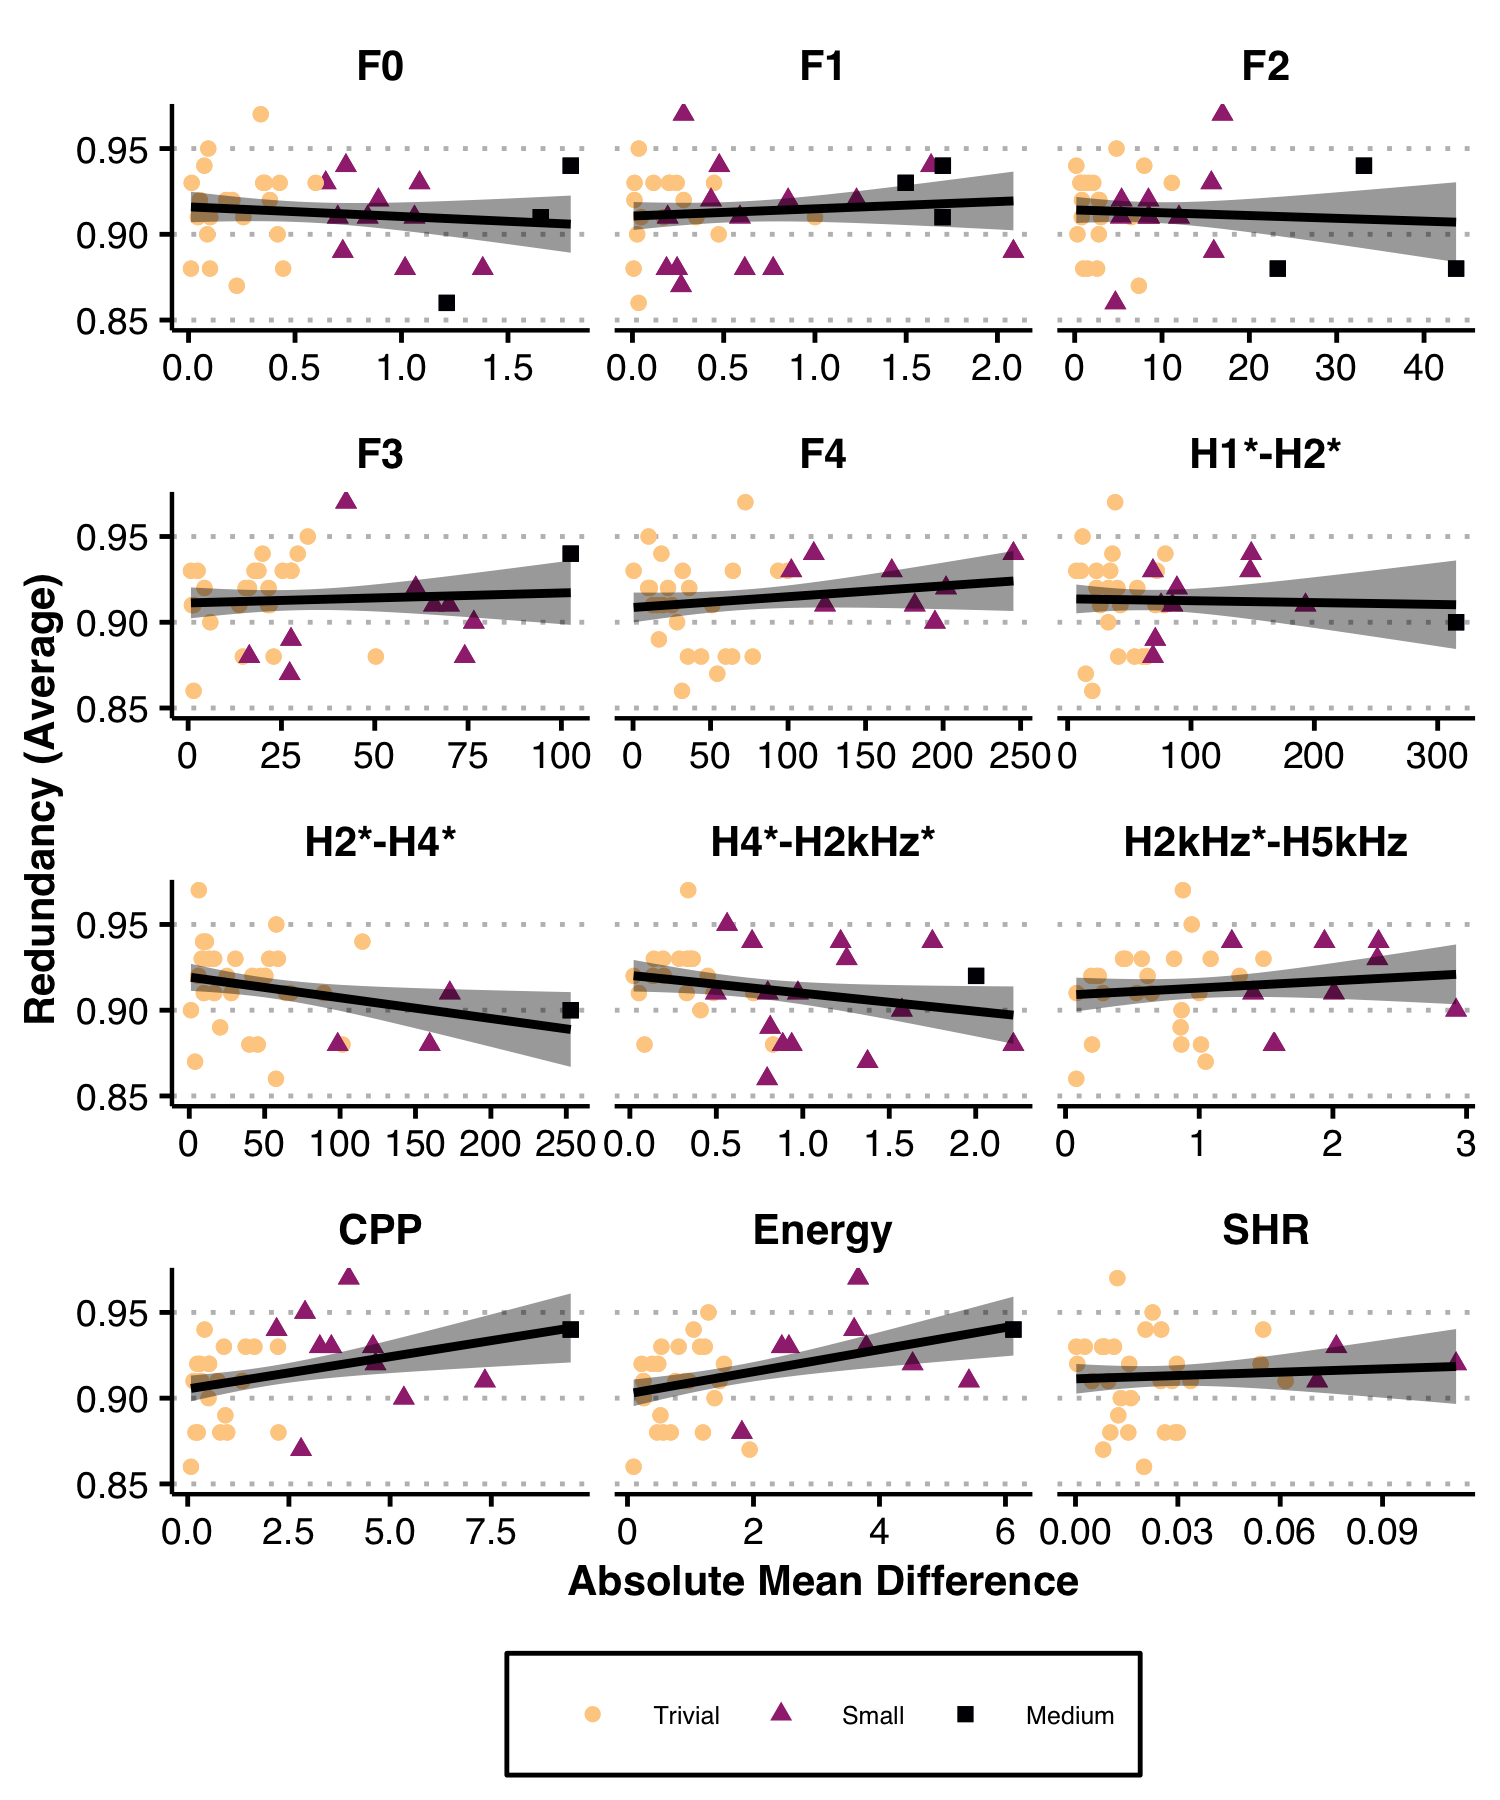
\includegraphics[width=0.85\linewidth]{figures/ch3_redundancybyttestdiff_5in.png} 
    \caption{This plot depicts the relationship between the absolute value of the difference of means from the t-tests, plotted against the average redundancy value for the talker. Color and shape indicate whether the Cohens' \textit{d} of the t-test was trivial, small, or medium. The superimposed regression line summarizes the relationship between these values. }
    \label{ch3:fig:diffbyred}
    \end{center}
\end{figure}

This high degree of similarity does not preclude crosslinguistic differences on a within-talker basis but rather suggests that such differences occur on a more global level. This is apparent in Figure \ref{ch3:fig:diffbyred}, which depicts the relationship between talkers' average redundancy from Section \ref{ch3:sec:cca} and the difference between the mean values for each of the acoustic measurements in Section \ref{ch3:sec:comparison}. If there were clear relationships between large crosslinguistic differences and redundancy, the regression lines should be strongly negative---this does not seem to be the case.

Such high similarity in the PCAs was not entirely expected, given the results of \citet{lee_2019_acoustic}, where a handful of shared components were evident but were complemented by numerous idiosyncratic components. At face value, the results in this chapter suggest that a heterogeneous bilingual population has more across-talker similarity than a tightly controlled group of monolingual English speakers. Several analysis decisions may have contributed to this apparent difference. I compared similar components independent of order, which ignores the fact that similar components may account for different amounts of variance, but ensures that comparisons are made among like items. Any downside to this methodological decision is mitigated by the fact that most components made relatively small contributions in how much of the overall variance they accounted for (see Table \ref{ch3:tab:componentcount}). As such, I predict that increased across-talker similarity would be found in a reanalysis of the UCLA Speaker Variability Database \citep{keating_2019_database} using the adapted methods of this chapter. 

While methodological choices may account for some part of these results, the data differences between the current chapter and previous studies are also pertinent. This chapter uses substantially longer passages than the short samples in \citet{lee_2019_acoustic}. Larger speech samples clearly allow for a stable underlying structure to emerge. Smaller samples, conversely, may reflect more ephemeral variation in a talker's voice, and thus not be representative of the talker's full range. The passage length analysis in this chapter shows that the number of samples needed for stabilization is substantially larger than the 5000 samples used in \citet{lee_2019_acoustic}. This does not necessarily discount their work, however, as the current chapter uses spontaneous speech, which is arguably more variable than read speech.\footnote{While it is true that \citet{} examined spontaneous speech, the poster only states that two minutes of speech were used for each participant. By this estimation, the sample size was likely on the lower side, compared to the 20-25 minute interviews in the SpiCE corpus. However, it is not possible to make a direct comparison without knowing the number of samples.} It's plausible that an analysis of sentence reading would not need as much data to cover talkers' range of variability in reading aloud. The body of literature in the introduction establishes differences in voice quality across speaking styles \citep[e.g.,][]{lee_2017_bilingual}. As such, the threshold suggested here may only be appropriate for the speaking style of peer-to-peer conversational interviews. In any case, the methods presented here offer a tool for researchers to use in assessing whether their sample size is representative of a larger whole. Understanding how this interacts with speaking style is left for future directions. 

Ultimately, the goal of this line of research is to understand how the acoustic variability and structure of talkers' voices maps onto listeners' organization of a voice space for use in talker recognition and discrimination. Turning to listener and behavioral data will help in deciphering what is meaningful variation within a voice from low-level noise that cannot be attributed to a particular vocal signature. Verification from listener performance will help adjudicate which statistical choices present an acoustic voice space that matches listener organization. The results of this chapter set up predictions for that work. These predictions will be revisited in general discussion.

\endinput % -------------------------------------------------------- %
